%\documentclass{beamer}
\documentclass[handout]{beamer}
\usetheme{Frankfurt}
\newcommand{\answers}{1}

\usepackage{amsmath}
\usepackage{caption}
\usepackage{color}
\usepackage{enumerate}
\usepackage{listings}
\usepackage{hyperref}
\usepackage{mathrsfs}
\usepackage{movie15}
\usepackage{natbib}
\usepackage{setspace}
\usepackage{tikz}
\usepackage{tkz-graph}
\usepackage{url}

\providecommand{\all}{\ \forall \ }
\providecommand{\bs}{\backslash}
\providecommand{\e}{\varepsilon}
\providecommand{\E}{\ \exists \ }
\providecommand{\lm}[2]{\lim_{#1 \rightarrow #2}}
\providecommand{\m}[1]{\mathbb{#1}}
\providecommand{\mc}[1]{\mathcal{#1}}
\providecommand{\nv}{{}^{-1}}
\providecommand{\ov}[1]{\overline{#1}}
\providecommand{\p}{\newpage}
\providecommand{\q}{$\quad$ \newline}
\providecommand{\rt}{\rightarrow}
\providecommand{\Rt}{\Rightarrow}
\providecommand{\vc}[1]{\boldsymbol{#1}}
\providecommand{\wh}[1]{\widehat{#1}}

\hypersetup{colorlinks,linkcolor=,urlcolor=blue}
\numberwithin{equation}{section}

\definecolor{dkgreen}{rgb}{0,0.6,0}
\definecolor{gray}{rgb}{0.5,0.5,0.5}
\definecolor{mauve}{rgb}{0.58,0,0.82}

\lstset{ 
  language=C,                % the language of the code
  basicstyle= \footnotesize,           % the size of the fonts that are used for the code
  numbers=left,
  numberfirstline=true,
  numbersep=5pt,                  % how far the line-numbers are from the code
  backgroundcolor=\color{white},      % choose the background color. You must add \usepackage{color}
  showspaces=false,               % show spaces adding particular underscores
  showstringspaces=false,         % underline spaces within strings
  showtabs=false,                 % show tabs within strings adding particular underscores
  frame=lrb,                   % adds a frame around the code
  rulecolor=\color{black},        % if not set, the frame-color may be changed on line-breaks within not-black text 
  tabsize=2,                      % sets default tabsize to 2 spaces
  captionpos=t,                   % sets the caption-position 
  breaklines=true,                % sets automatic line breaking
  breakatwhitespace=false,        % sets if automatic breaks should only happen at whitespace
  %title=\lstname,                   % show the filename of files included with \lstinputlisting;
  keywordstyle=\color{blue},          % keyword style
  commentstyle=\color{gray},       % comment style
  stringstyle=\color{dkgreen},         % string literal style
  escapeinside={\%*}{*)},            % if you want to add LaTeX within your code
  morekeywords={*, ...},               % if you want to add more keywords to the set
  xleftmargin=0.053in, % left horizontal offset of caption box
  xrightmargin=-.03in % right horizontal offset of caption box
}

\DeclareCaptionFont{white}{\color{white}}
\DeclareCaptionFormat{listing}{\parbox{\textwidth}{\colorbox{gray}{\parbox{\textwidth}{#1#2#3}}}}
\captionsetup[lstlisting]{format = listing, labelfont = white, textfont = white}
 %For caption-free listings, comment out the 3 lines above
 \lstset{frame = single}

\title{GPU-parallel Gibbs sampling of a hierarchical model of hybrid vigor in RNA-seq experiments}
\author{Will Landau}
\date{October 10, 2013}
\institute{Iowa State University}

\begin{document}

\setcounter{subsection}{1}
\begin{frame}
\titlepage
 \end{frame}
 
\begin{frame}
\frametitle{Outline}
\tableofcontents
\end{frame}

 \AtBeginSection[]
{
   \begin{frame}
       \frametitle{Outline}
       \tableofcontents[currentsection]
   \end{frame}
}



\section{Biological background}


%\subsection{DNA and RNA}


%\begin{frame}
%\frametitle{DNA}
%\begin{center}
%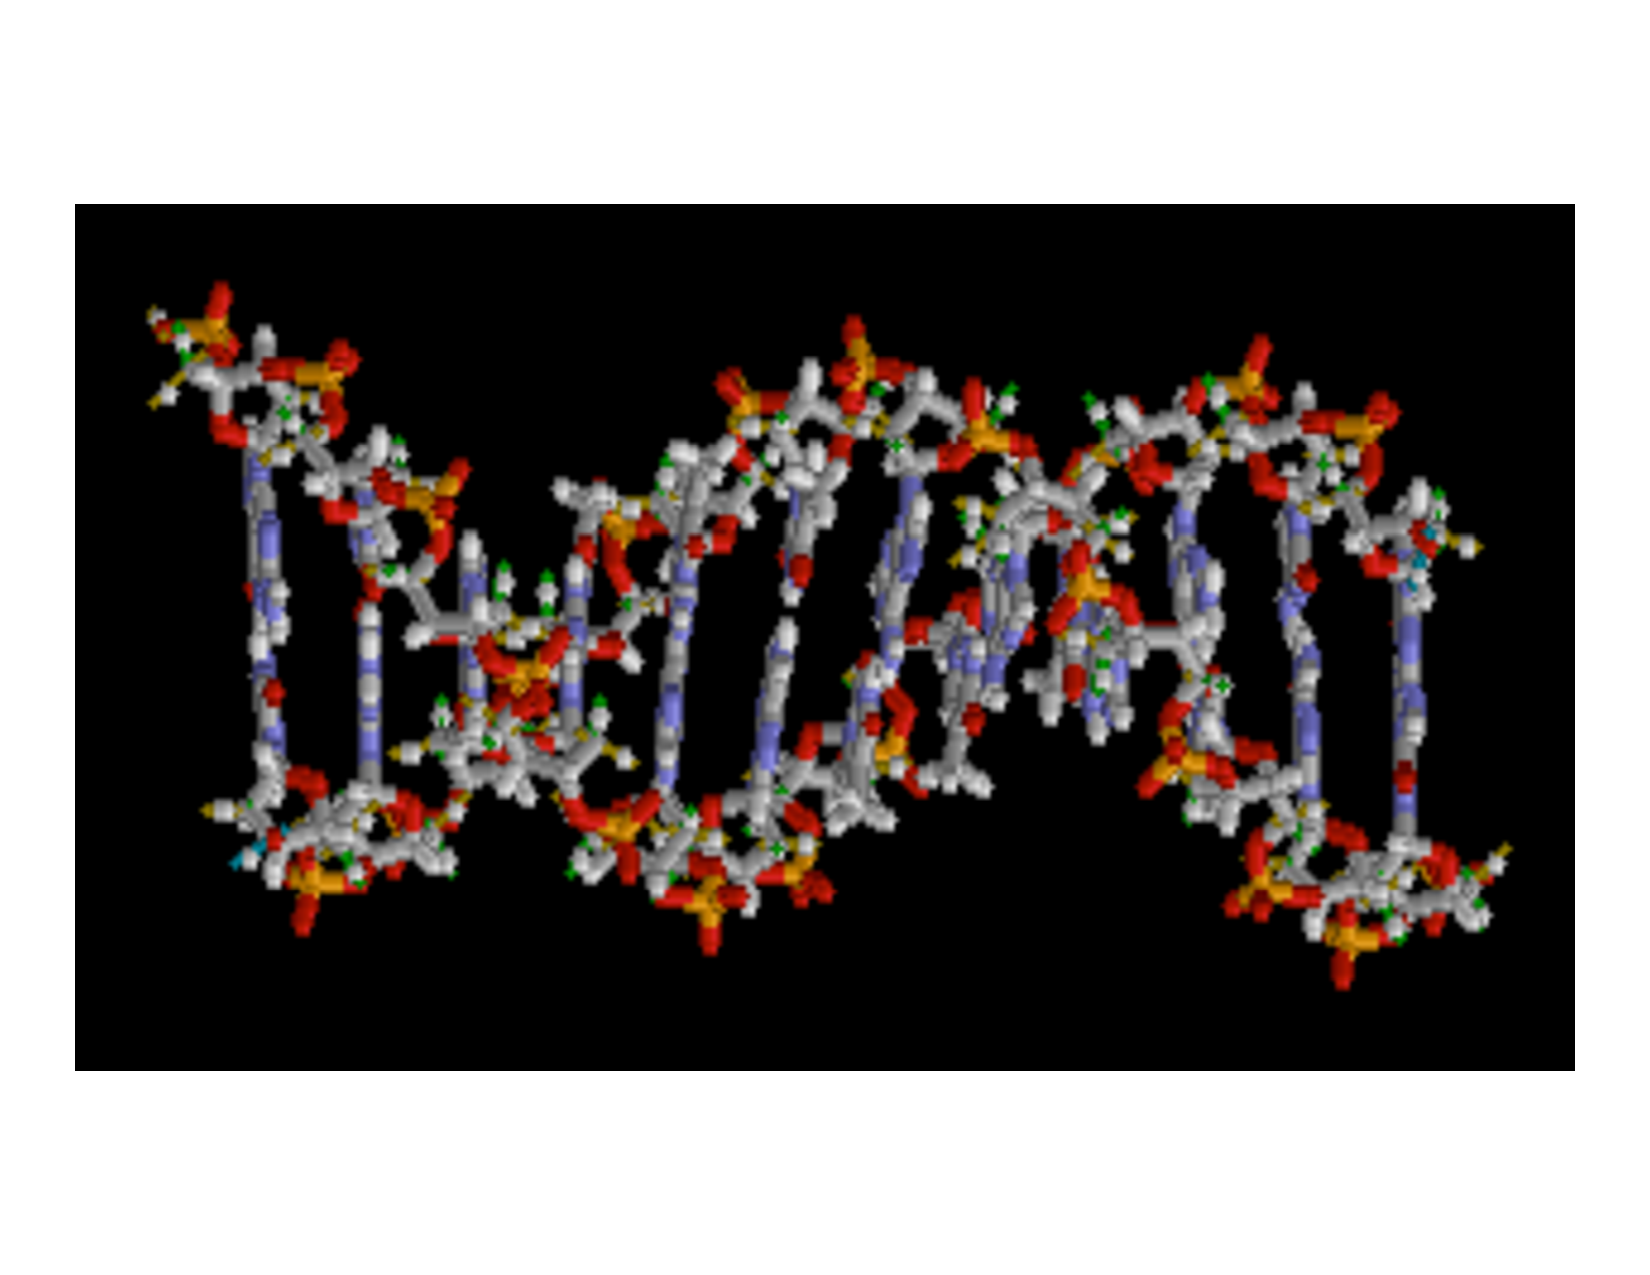
\includegraphics[scale=.23]{fig/dna-img}
%\end{center}
%\begin{center}
%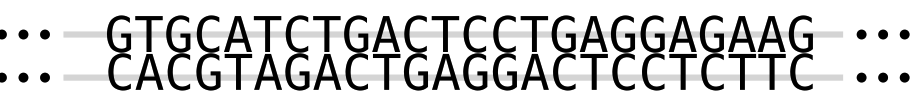
\includegraphics[scale=.23]{fig/dna.png}
%\end{center}
%\end{frame}


%\begin{frame}
%\frametitle{RNA}
%\begin{center}
%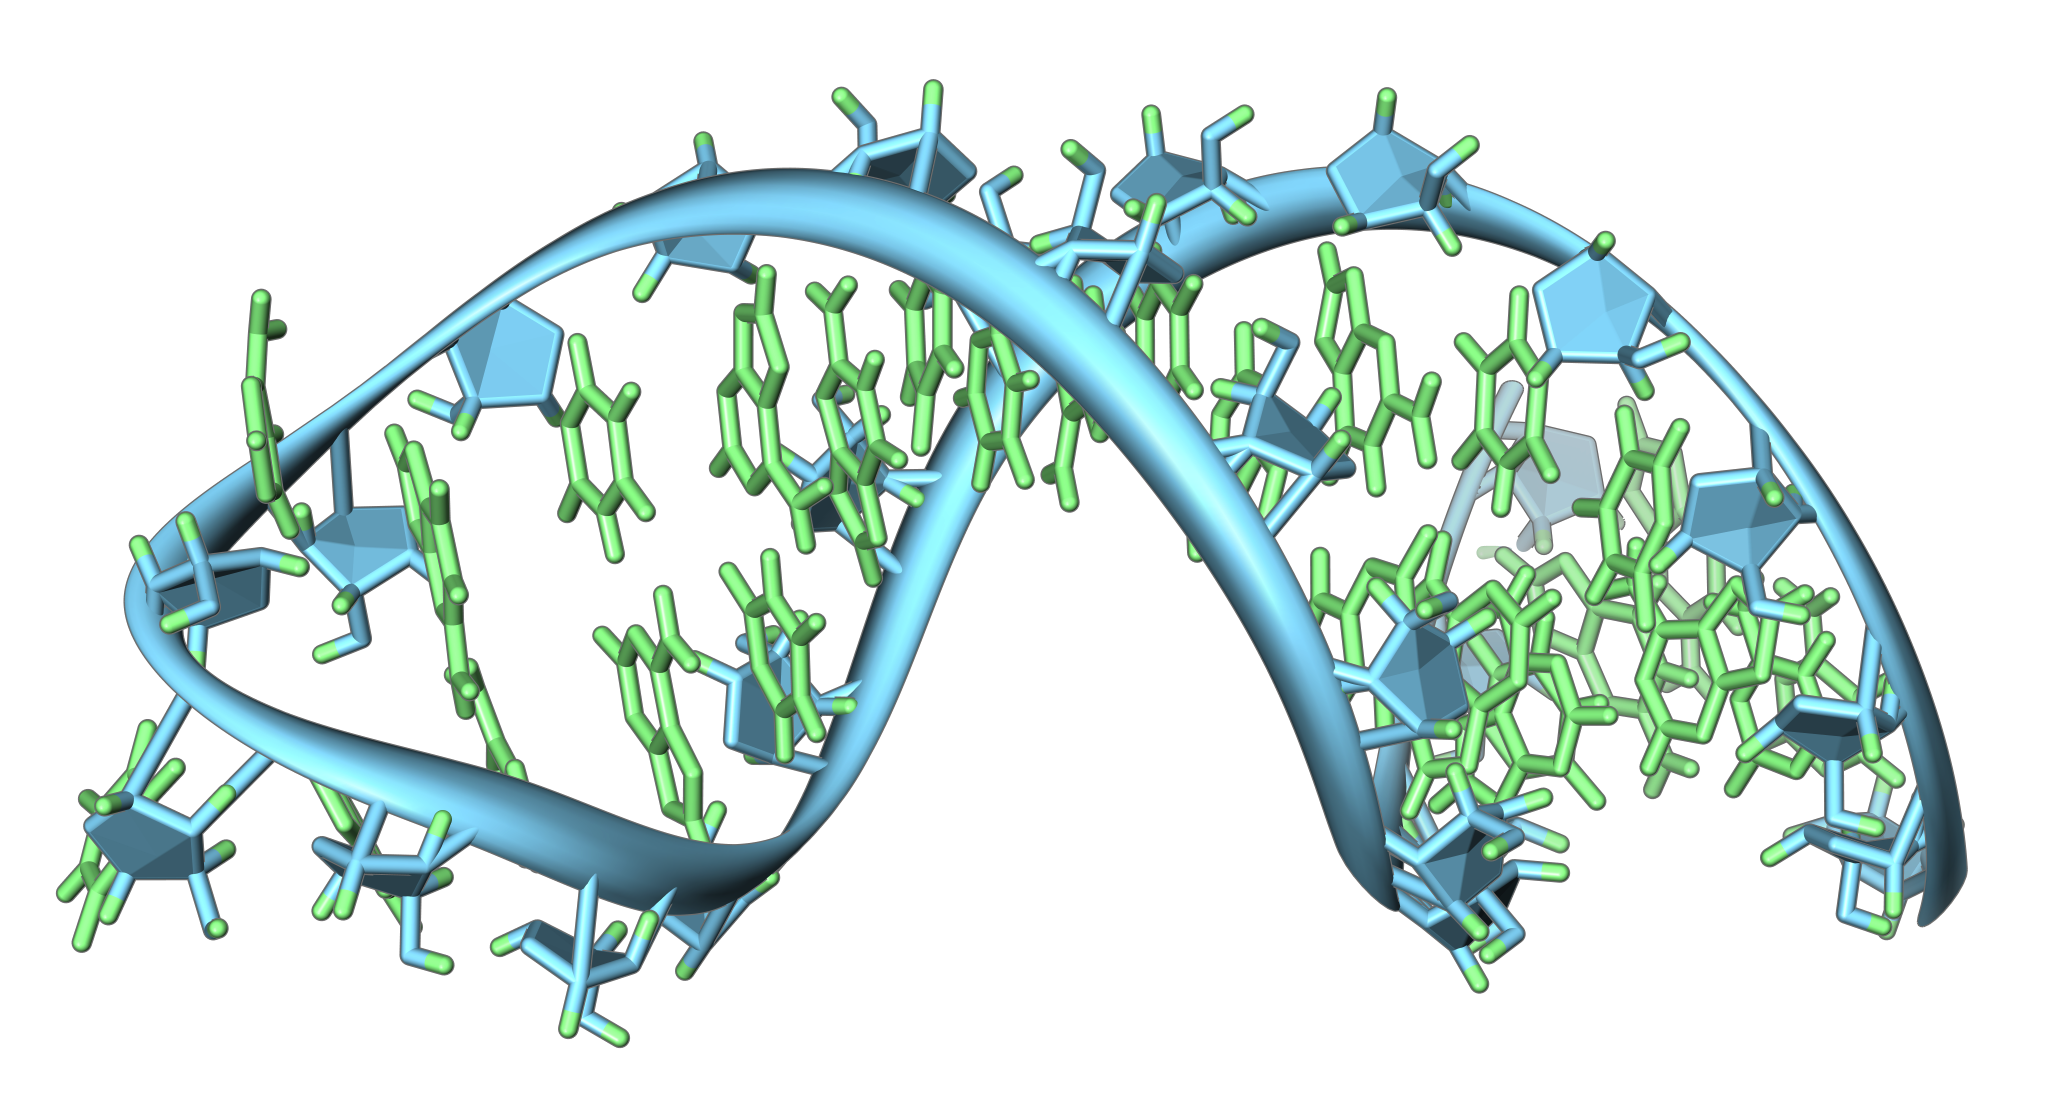
\includegraphics[scale=.07]{fig/rna-img.png}
%\end{center}
%\begin{center}
%
\includegraphics[scale=.23]{fig/rna.png}
%\end{center}
%\end{frame}


%\begin{frame}
%\frametitle{Proteins}
%\begin{center}
%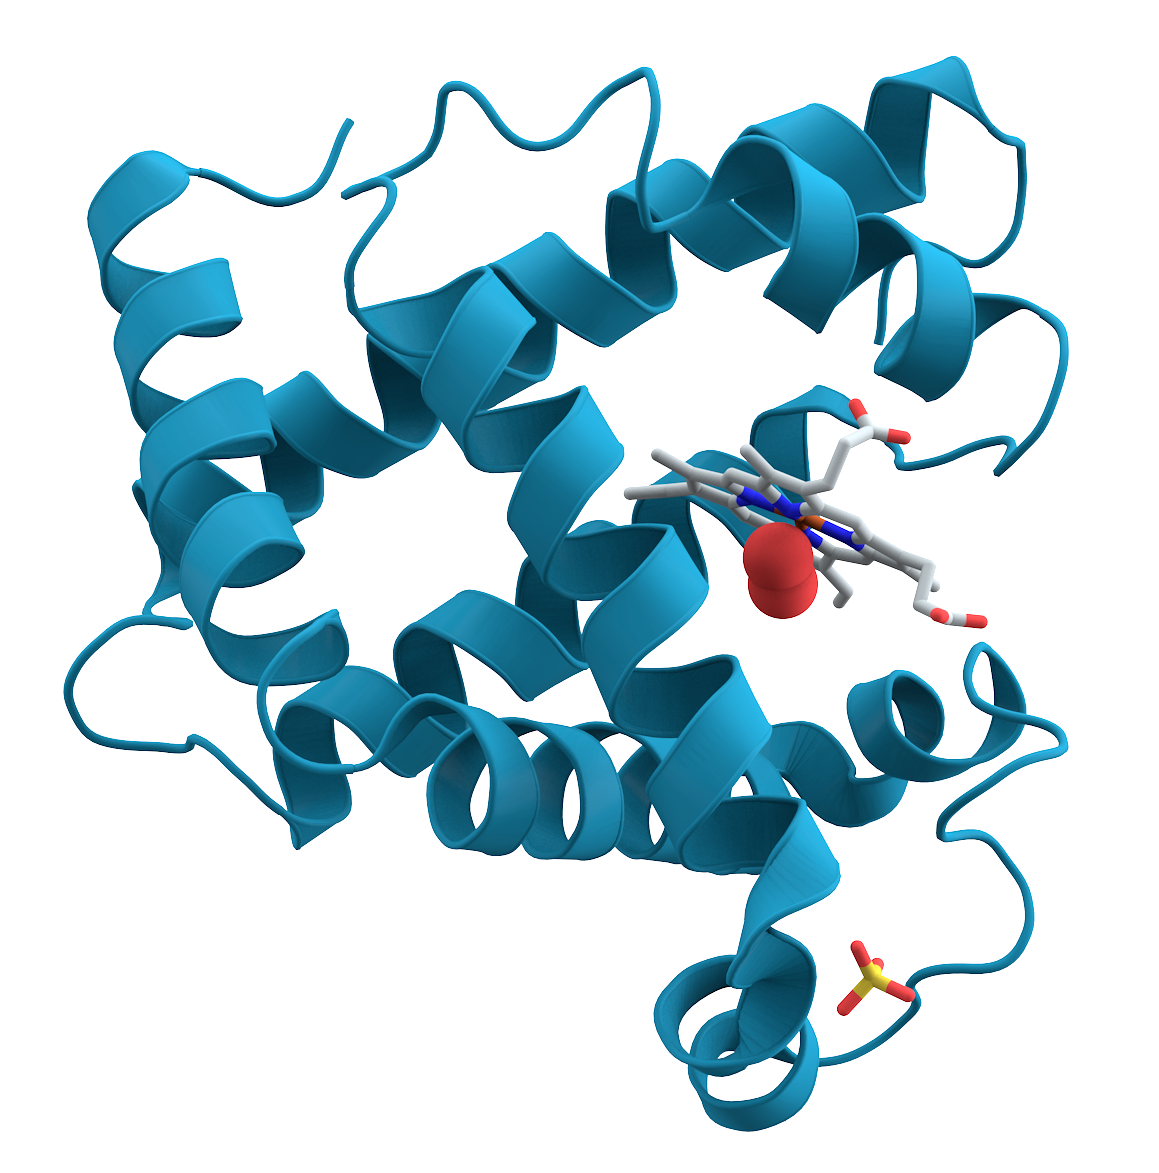
\includegraphics[scale=.07]{fig/myo.png}
%\end{center}
%\begin{center}
%
\includegraphics[scale=.23]{fig/protein.png}
%\end{center}
%\end{frame}

%\subsection{Central dogma}


%\begin{frame}
%\frametitle{Central dogma: how organisms make proteins}
%\begin{center}
%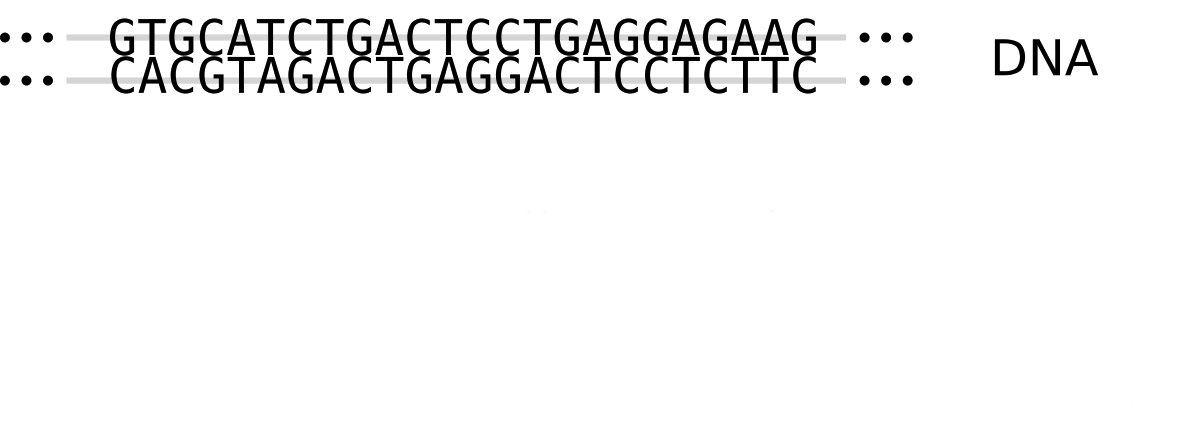
\includegraphics[scale=.23]{fig/dogma1.png}
%\end{center}
%\end{frame}

%\begin{frame}
%\frametitle{Central dogma: how organisms make proteins}
%\begin{center}
%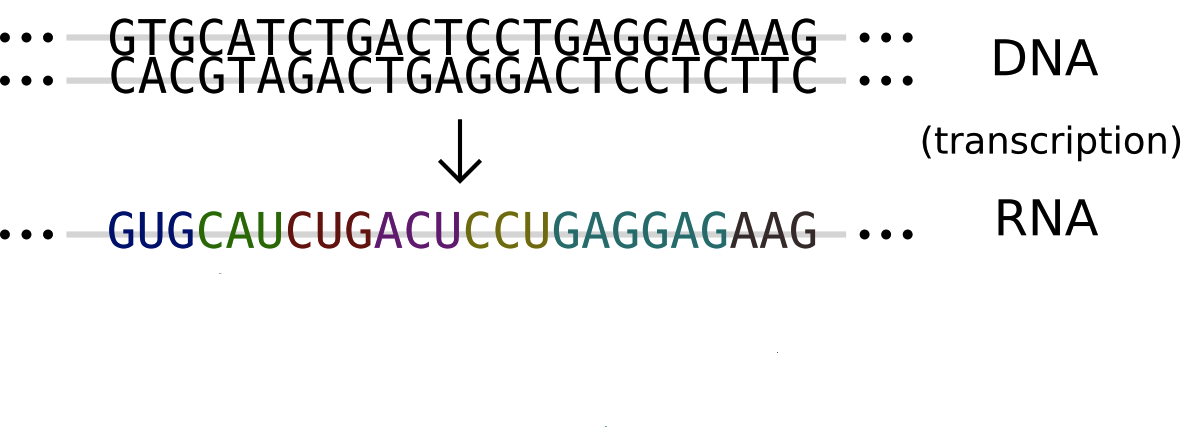
\includegraphics[scale=.23]{fig/dogma2.png}
%\end{center}
%\end{frame}


%\begin{frame}
%\frametitle{Central dogma of genetics}
%\begin{center}
%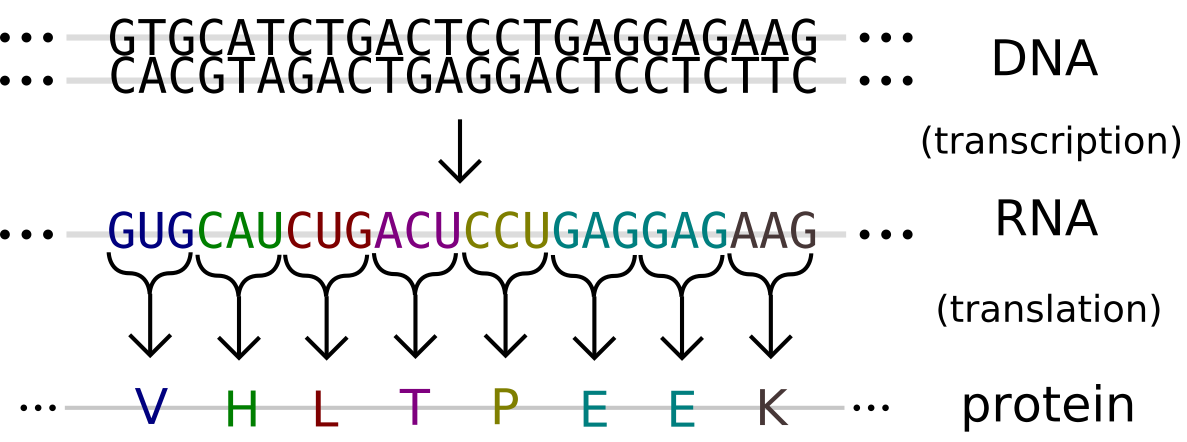
\includegraphics[scale=.23]{fig/dogma3.png}
%\end{center}
%\end{frame}

%\subsection{Examples of gene regulation}

%\begin{frame}
%\frametitle{HSP60}

%\begin{itemize}
%\item HSP = heat shock protein. 
%\item Prevent heat damage to other proteins.
%\end{itemize}
%\begin{center}
%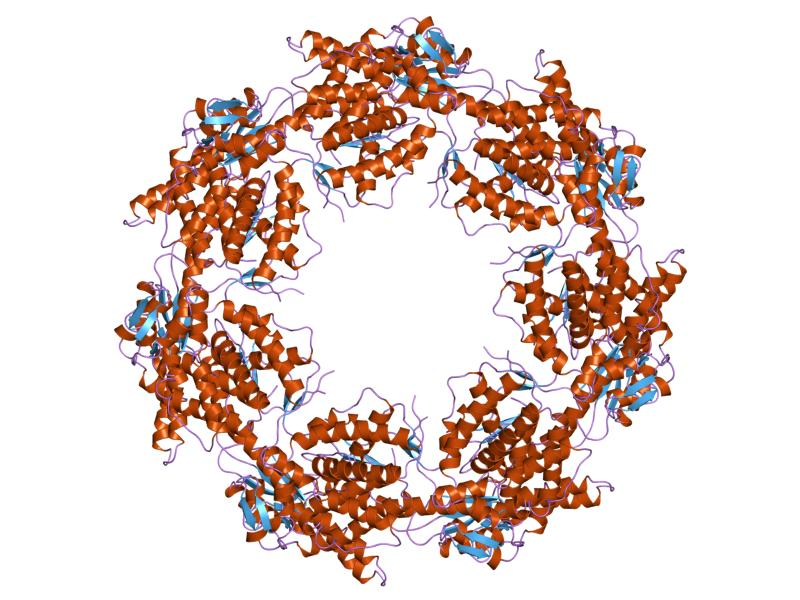
\includegraphics[scale=.23]{fig/hsp60.jpg}
%\end{center}
%\end{frame}

%\begin{frame}
%\frametitle{Temperature spike triggers HSP60 production.}
%\begin{center}
%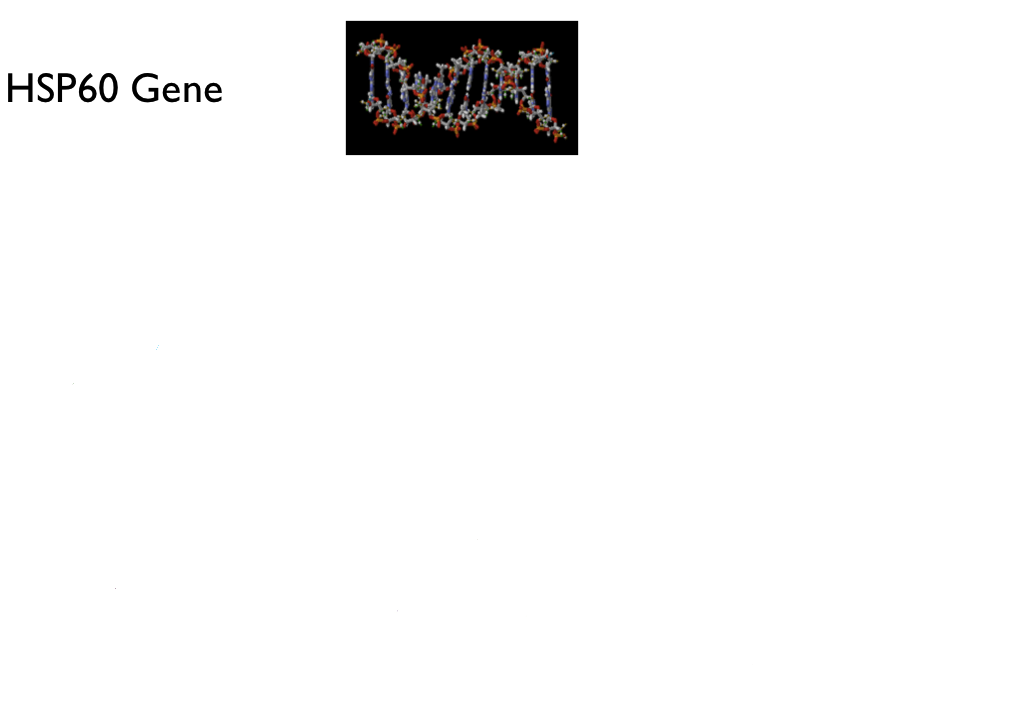
\includegraphics[scale=.25]{fig/hspt1.png}
%\end{center}
%\end{frame}

%\begin{frame}
%\frametitle{Temperature spike causes HSP60 expression.}
%\begin{center}
%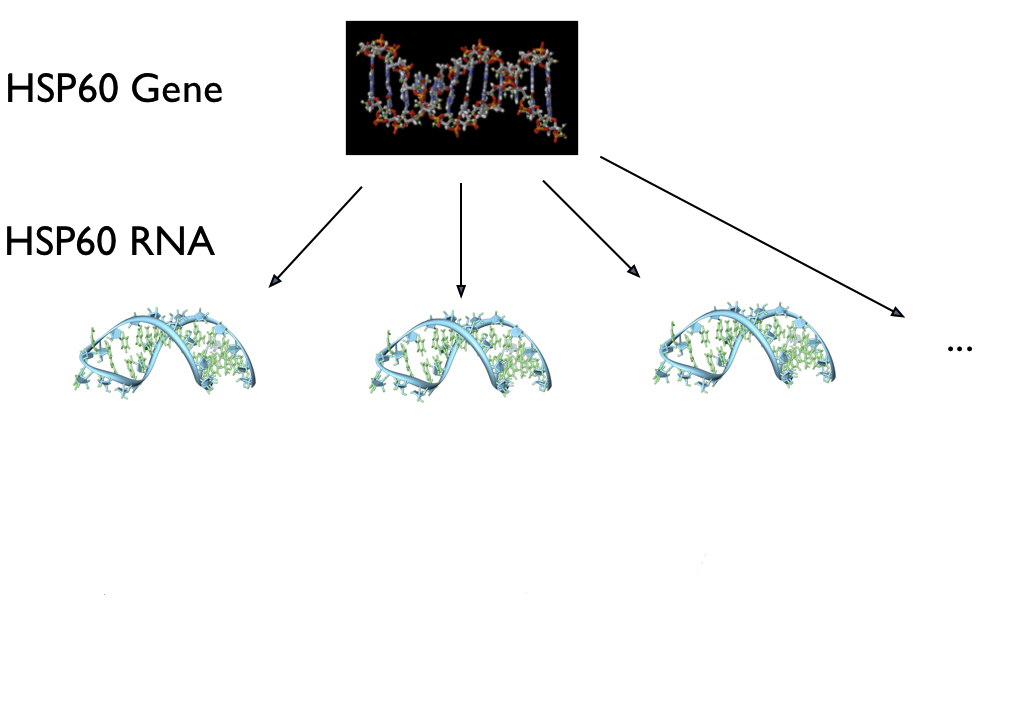
\includegraphics[scale=.25]{fig/hspt2.png}
%\end{center}
%\end{frame}

%\begin{frame}
%\frametitle{Temperature spike causes HSP60 expression.}
%\begin{center}
%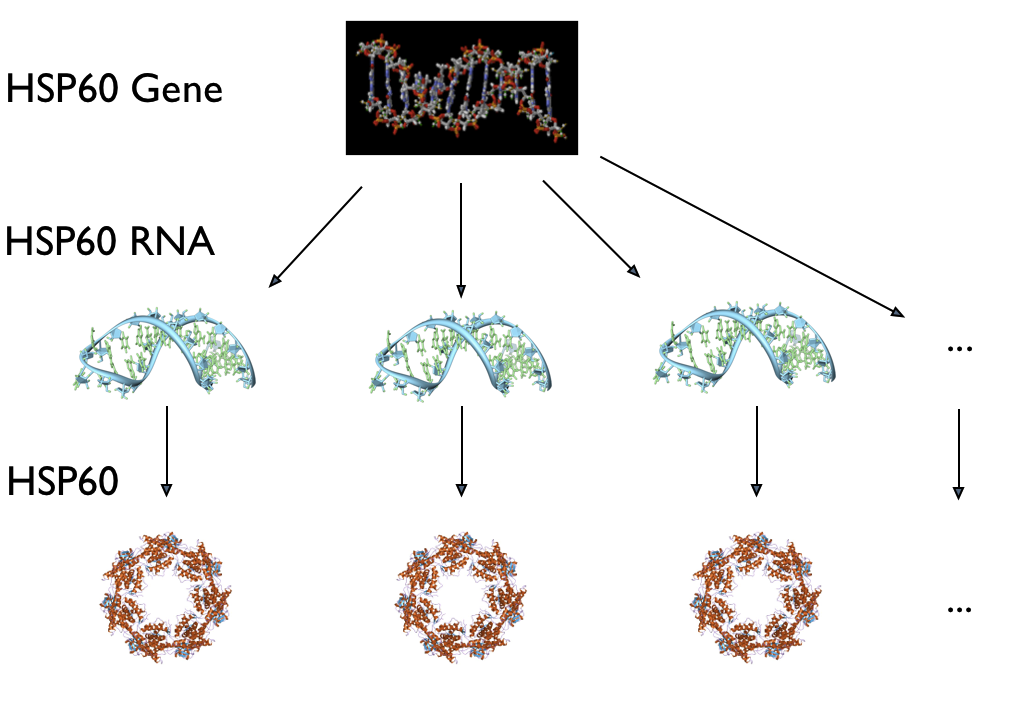
\includegraphics[scale=.25]{fig/hspt3.png}
%\end{center}
%\end{frame}


%\subsection{RNA-seq}


%\begin{frame}
%\frametitle{RNA-seq}

%\begin{itemize}
%\item RNA sequencing: measure gene expression using relative abundance of RNA.
%\item Illumina Genome Analyzer:
%\end{itemize}

%\begin{center}
%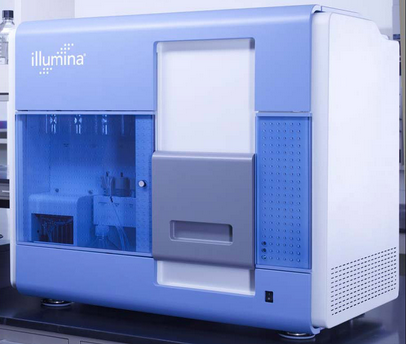
\includegraphics[scale=.35]{fig/illumina.png} $/ $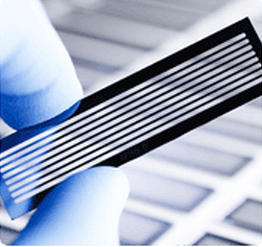
\includegraphics[scale=.45]{fig/flowcell.png}
%\end{center}
%\end{frame}



%\begin{frame}
%\frametitle{RNA-seq data: counts of amplified RNA fragments}
%%\begin{center}
%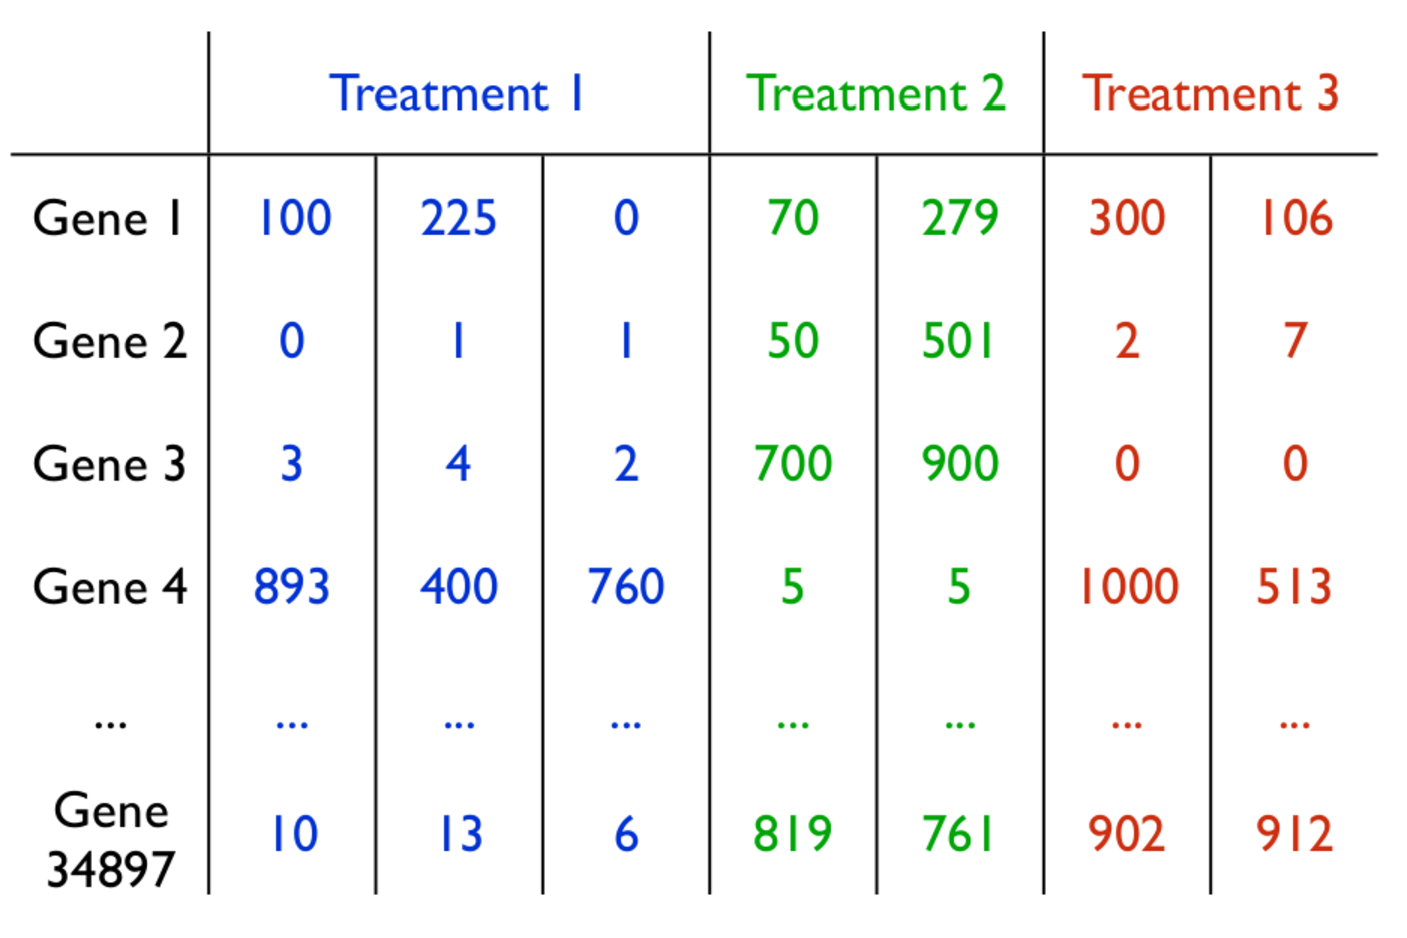
\includegraphics[scale=.35]{fig/rnaseqdata}
%\end{center}

%\begin{itemize}
%\item Goal: use RNA-seq to study hybrid vigor (heterosis).
%\end{itemize}

%\end{frame}




\subsection{Hybrid vigor}


\begin{frame}
\frametitle{High-parent heterosis: child's trait surpasses both parents}
\begin{center}
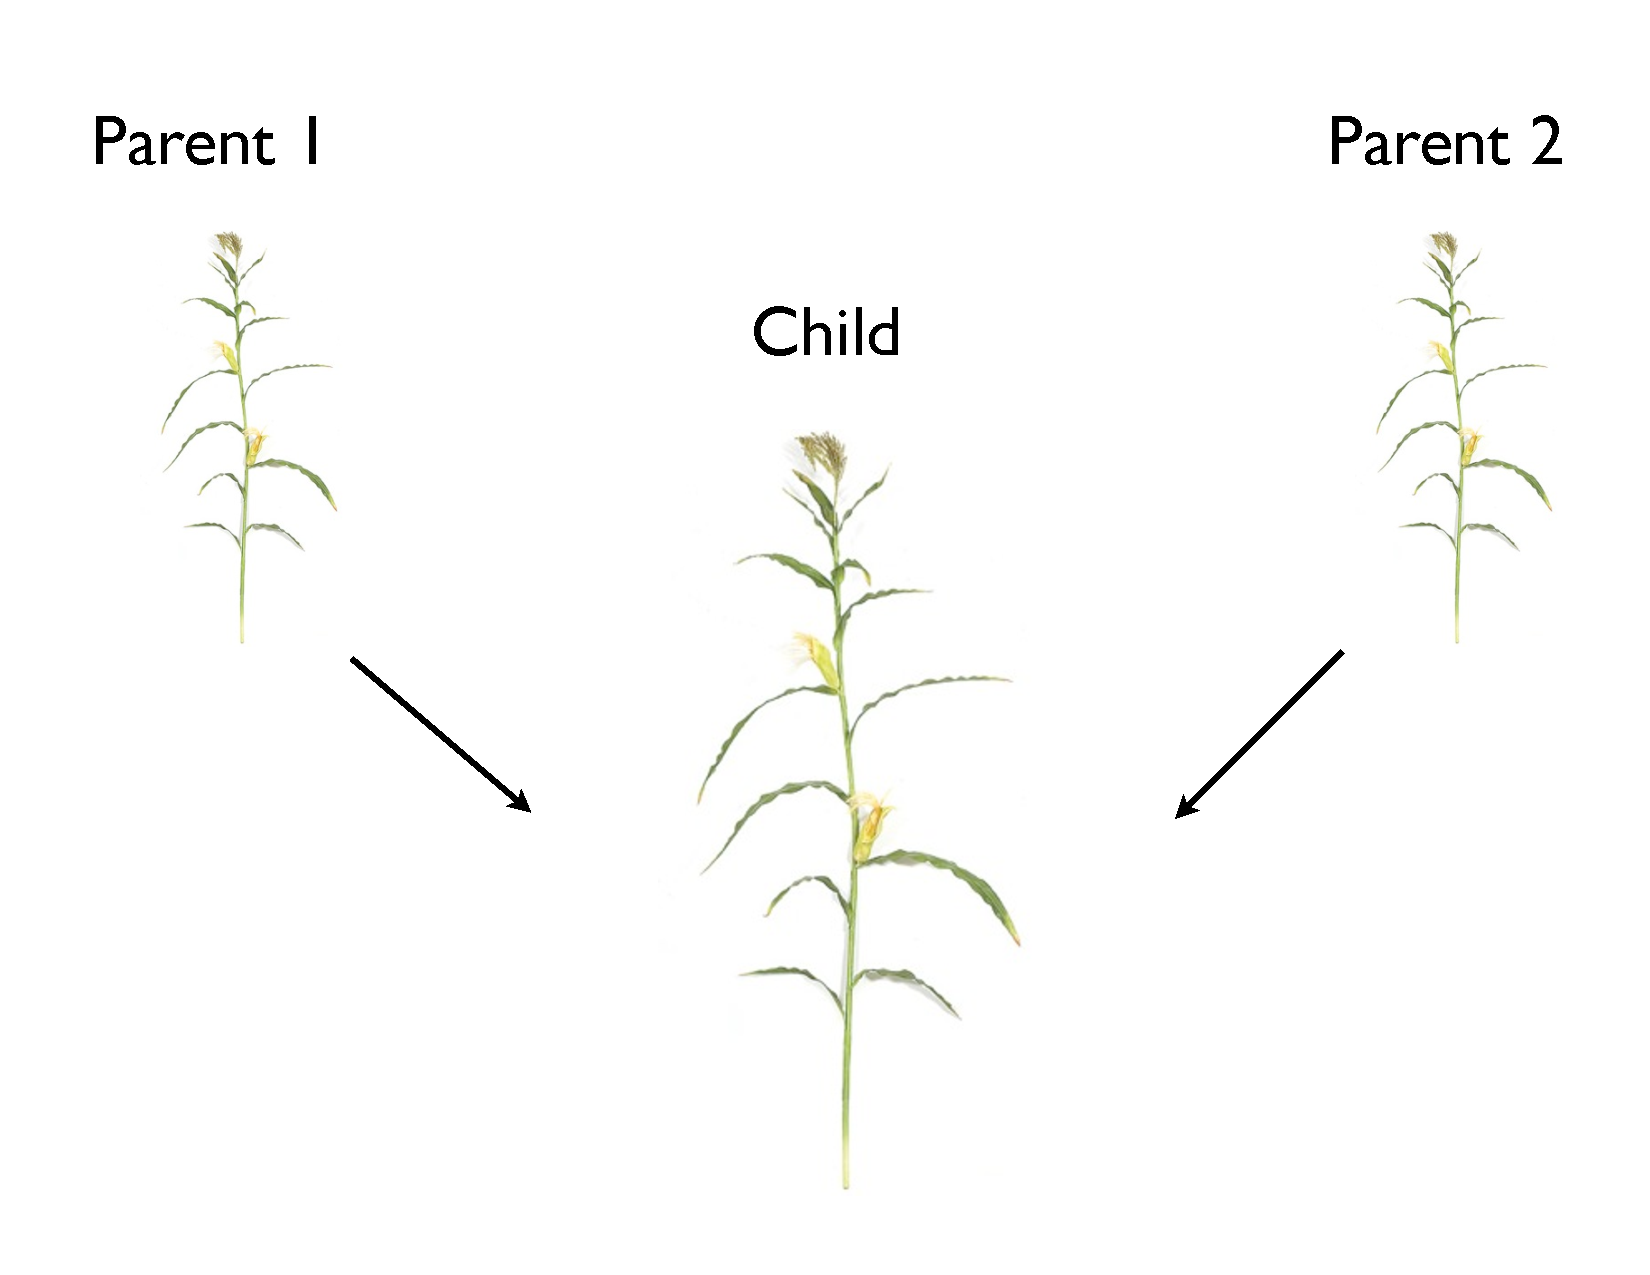
\includegraphics[scale=.3]{fig/hph}
\end{center}
\end{frame}


\begin{frame}
\frametitle{Low-parent heterosis: child's trait is weaker than in each parent}
\begin{center}
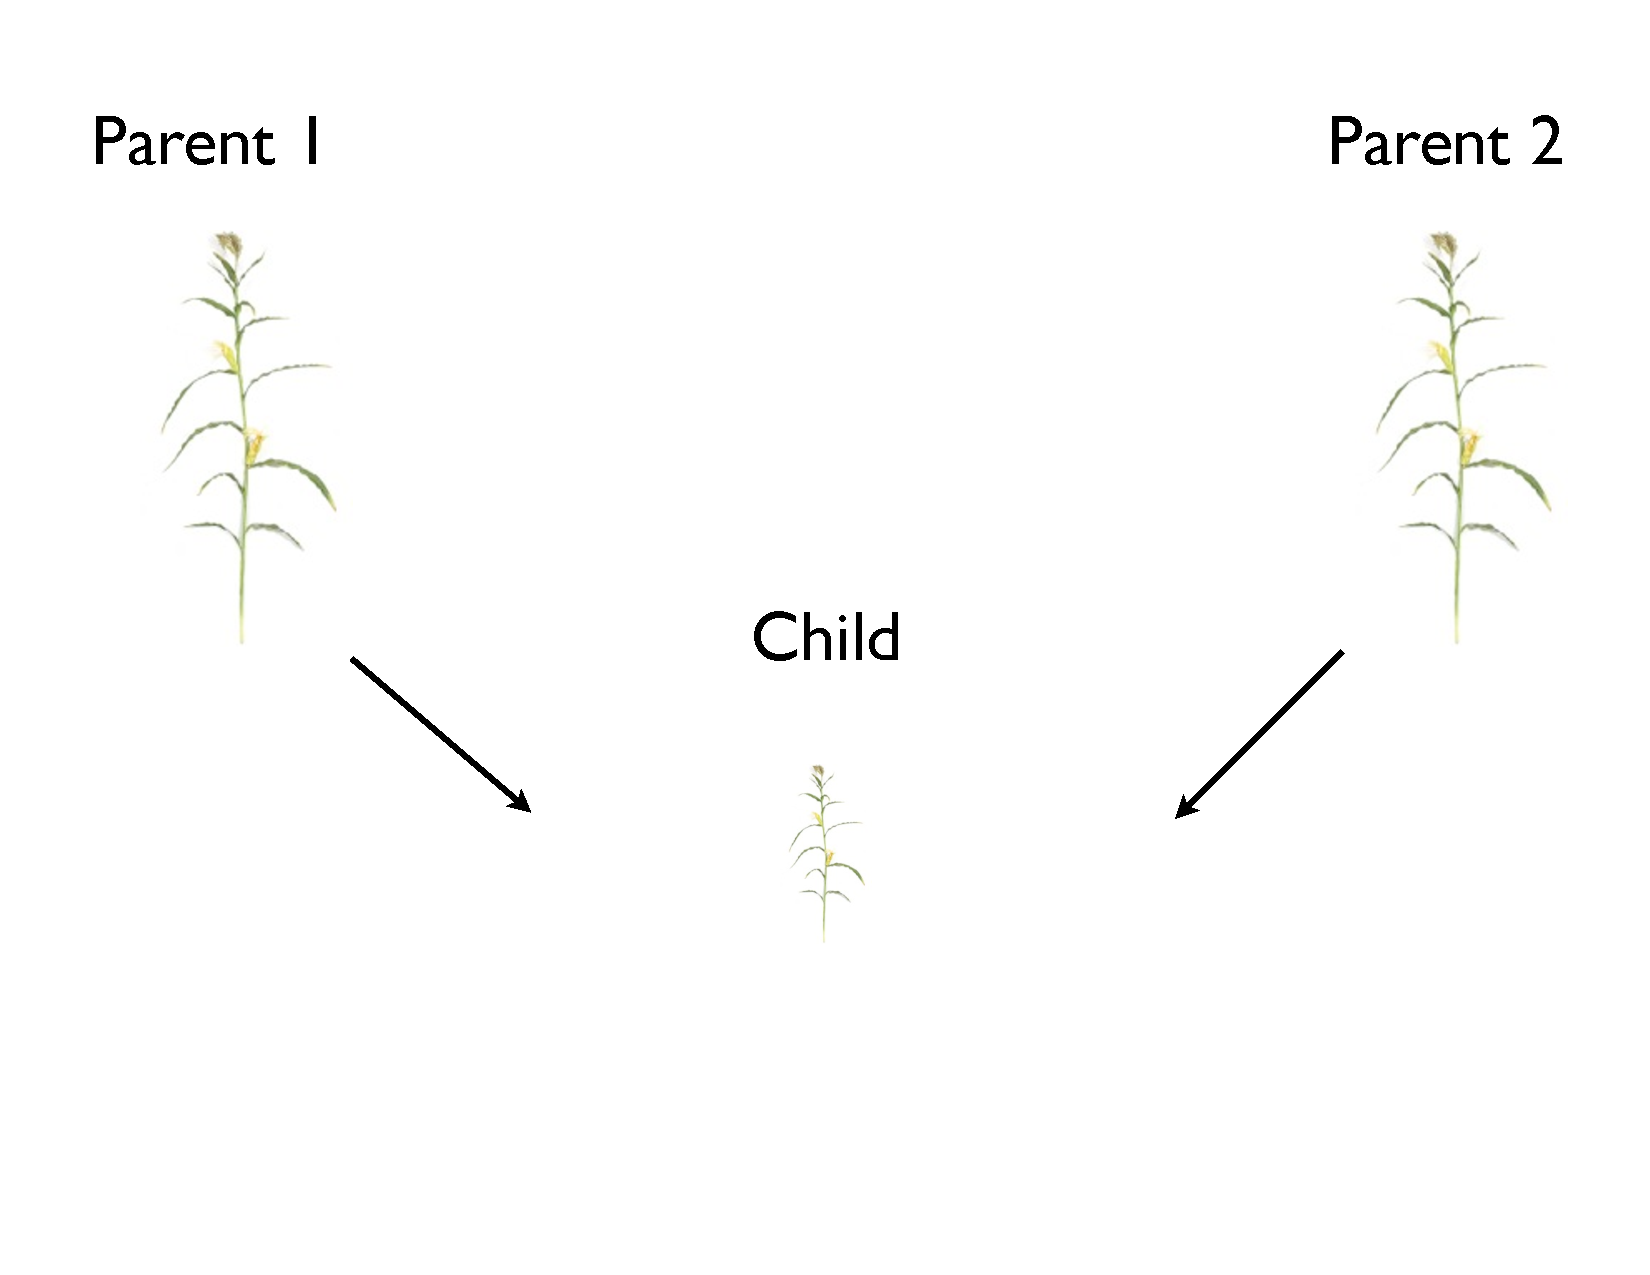
\includegraphics[scale=.3]{fig/lph}
\end{center}
\end{frame}


\begin{frame}
\frametitle{Mid-parent heterosis: child's trait is different than average of parents}
\begin{center}
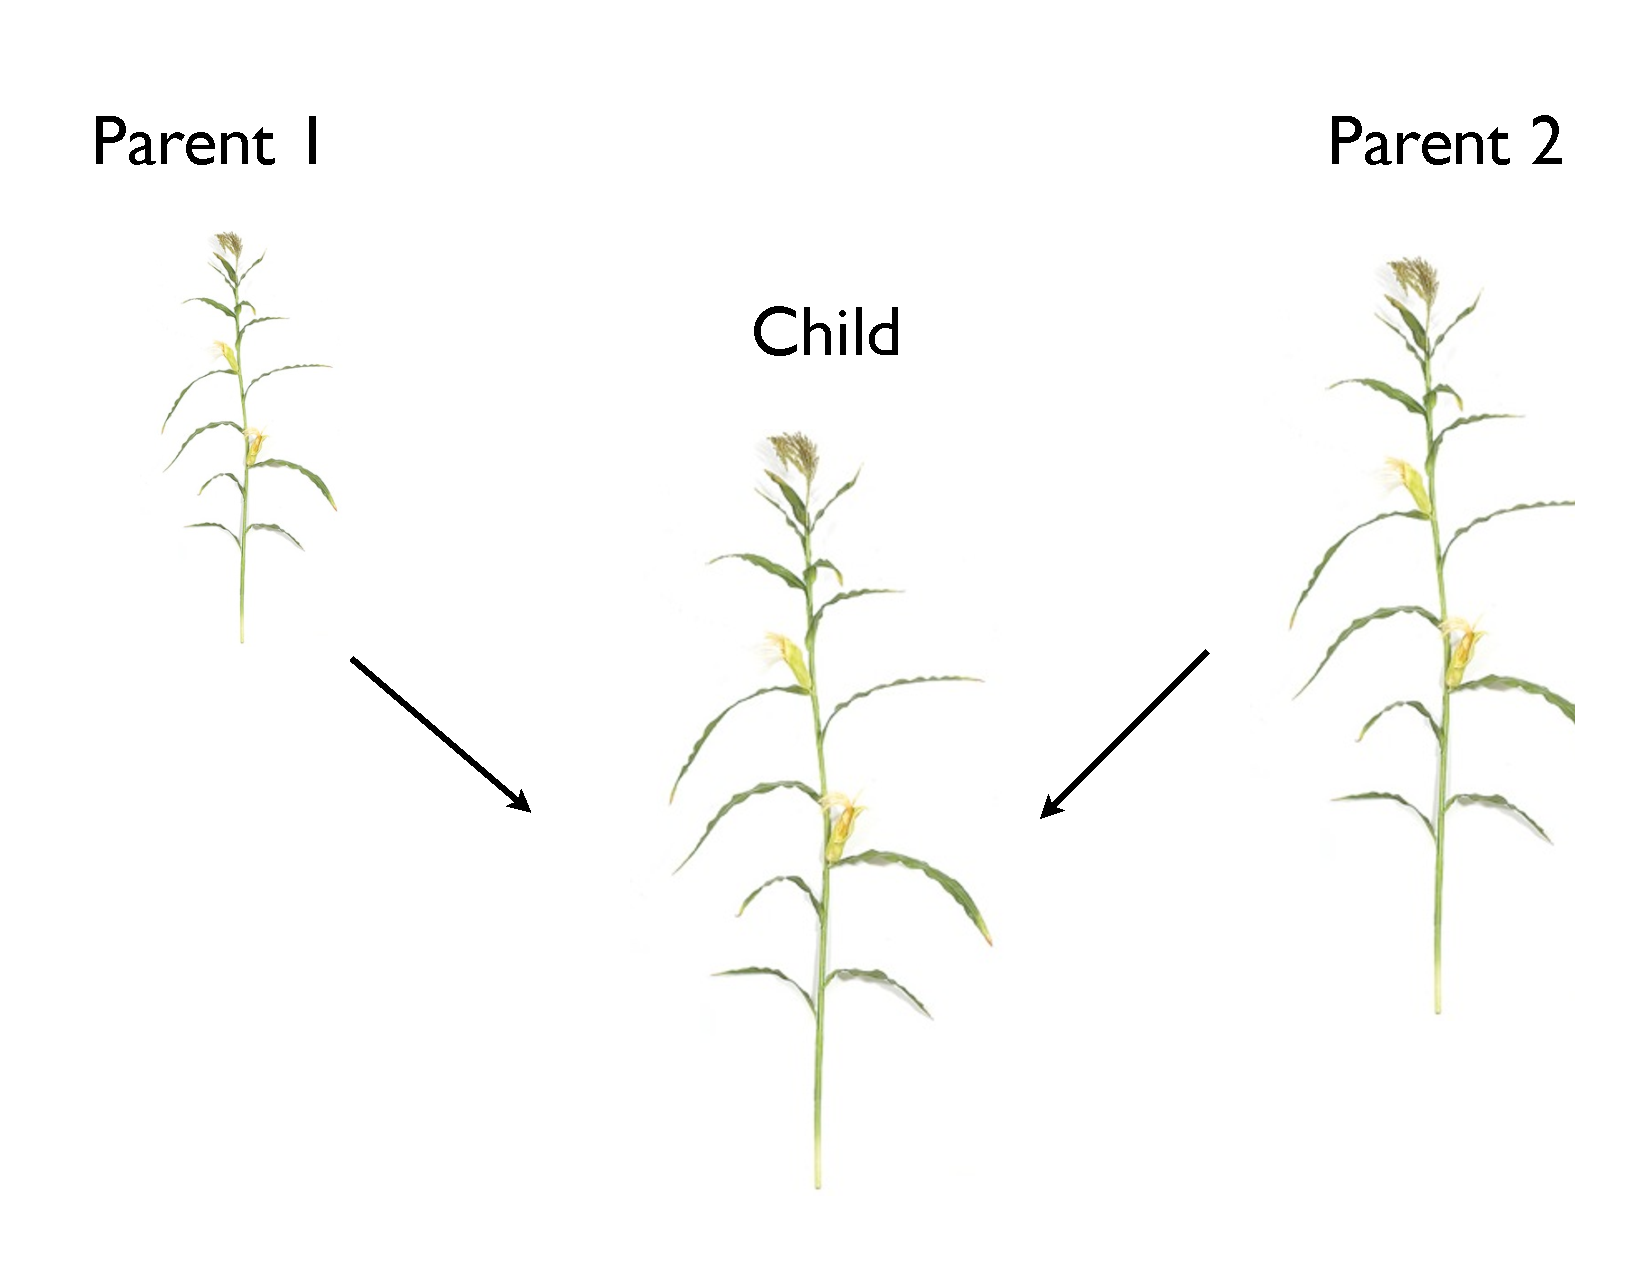
\includegraphics[scale=.3]{fig/mph}
\end{center}
\end{frame}



\begin{frame}
\frametitle{High-parent heterosis in gene expression}
\begin{center}
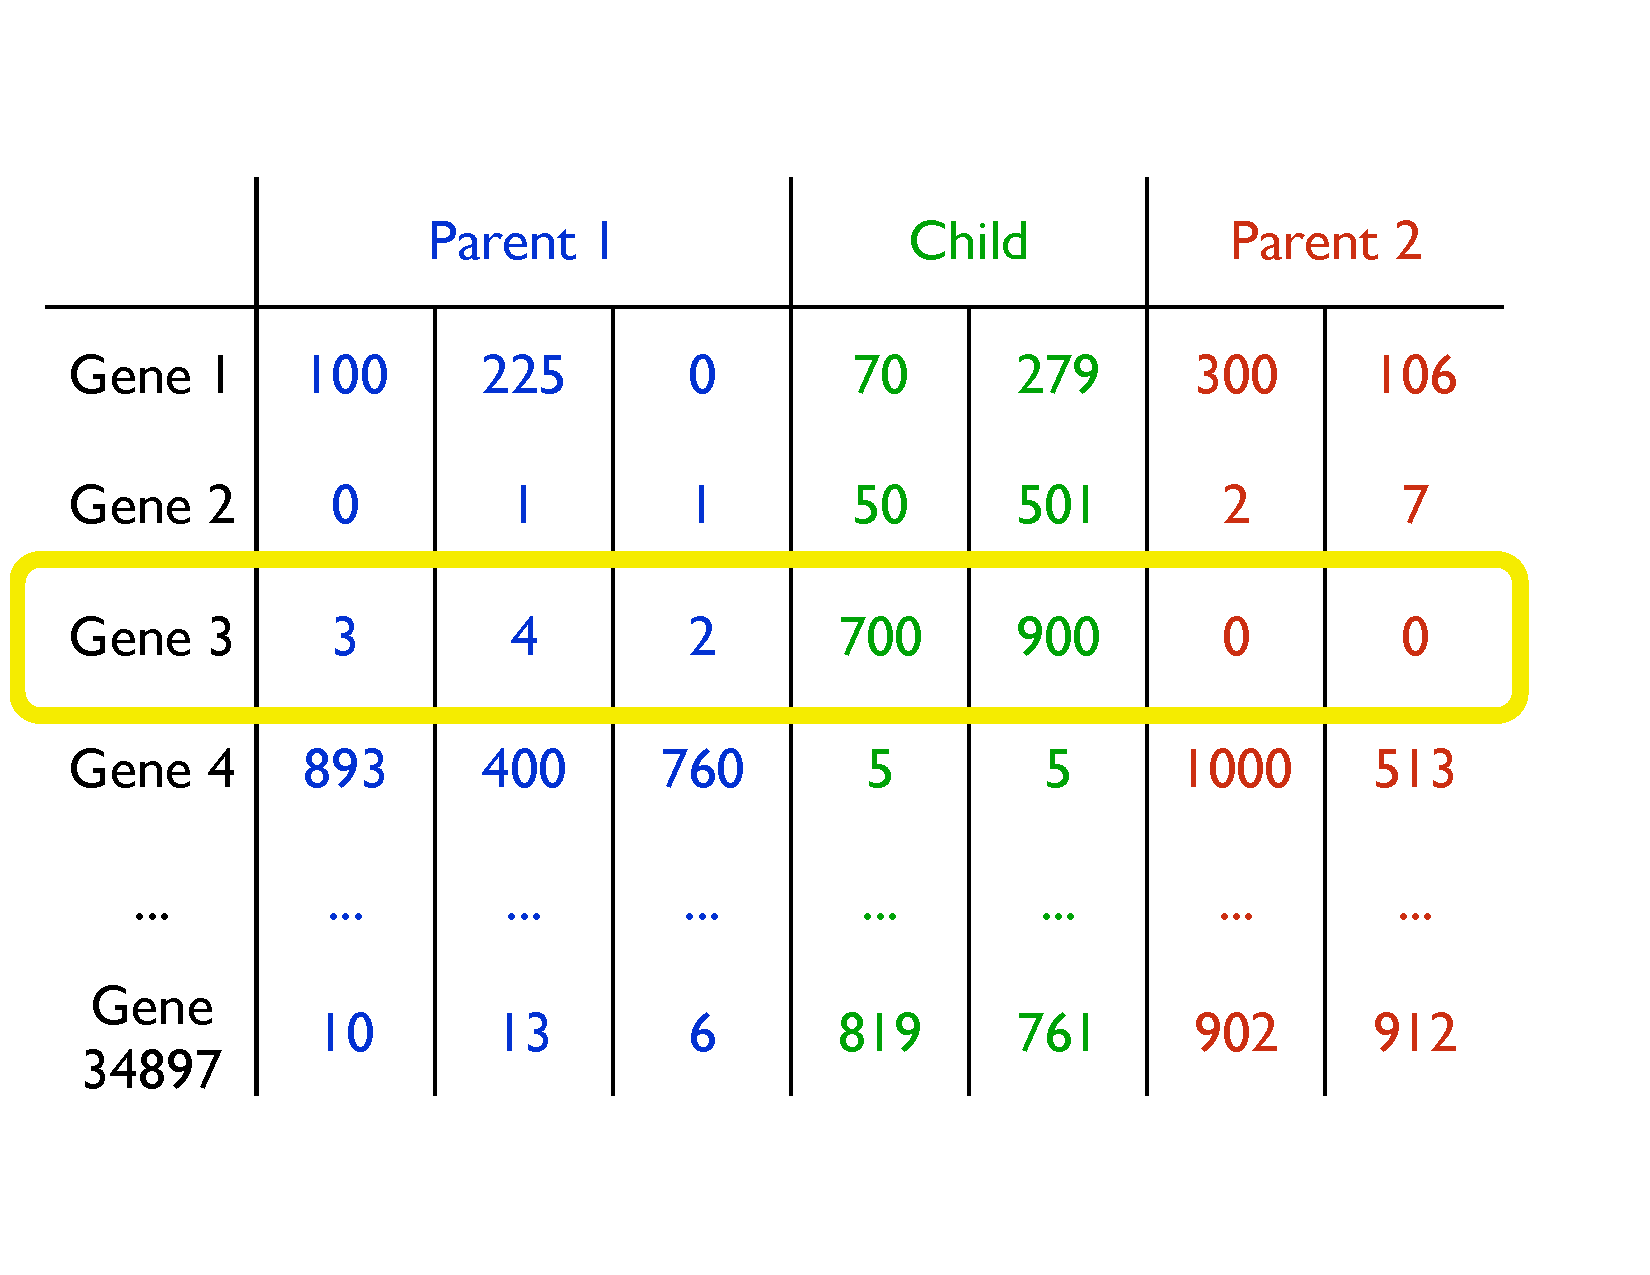
\includegraphics[scale=.35]{fig/hphrnaseq}
\end{center}
\end{frame}

\begin{frame}
\frametitle{Low-parent heterosis in gene expression}
\begin{center}
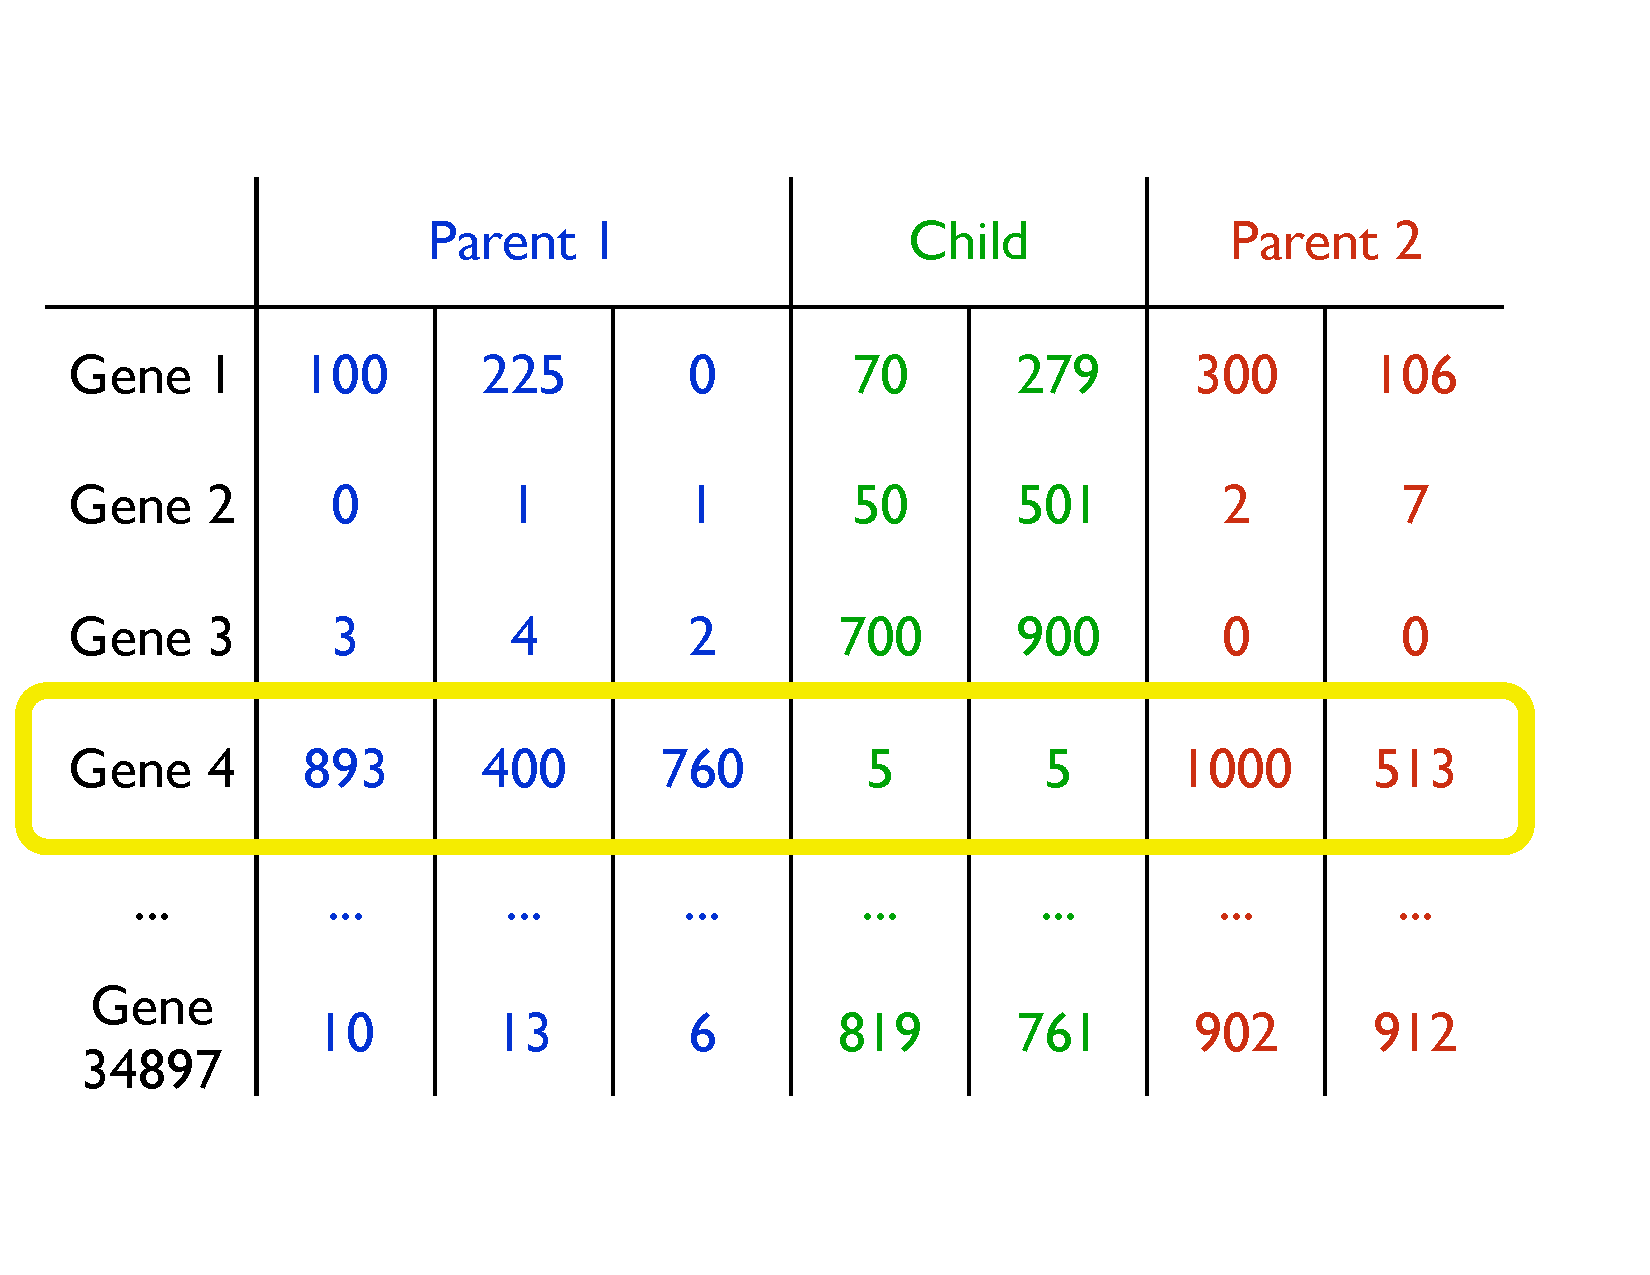
\includegraphics[scale=.35]{fig/lphrnaseq}
\end{center}
\end{frame}

\begin{frame}
\frametitle{Mid-parent heterosis in gene expression}
\begin{center}
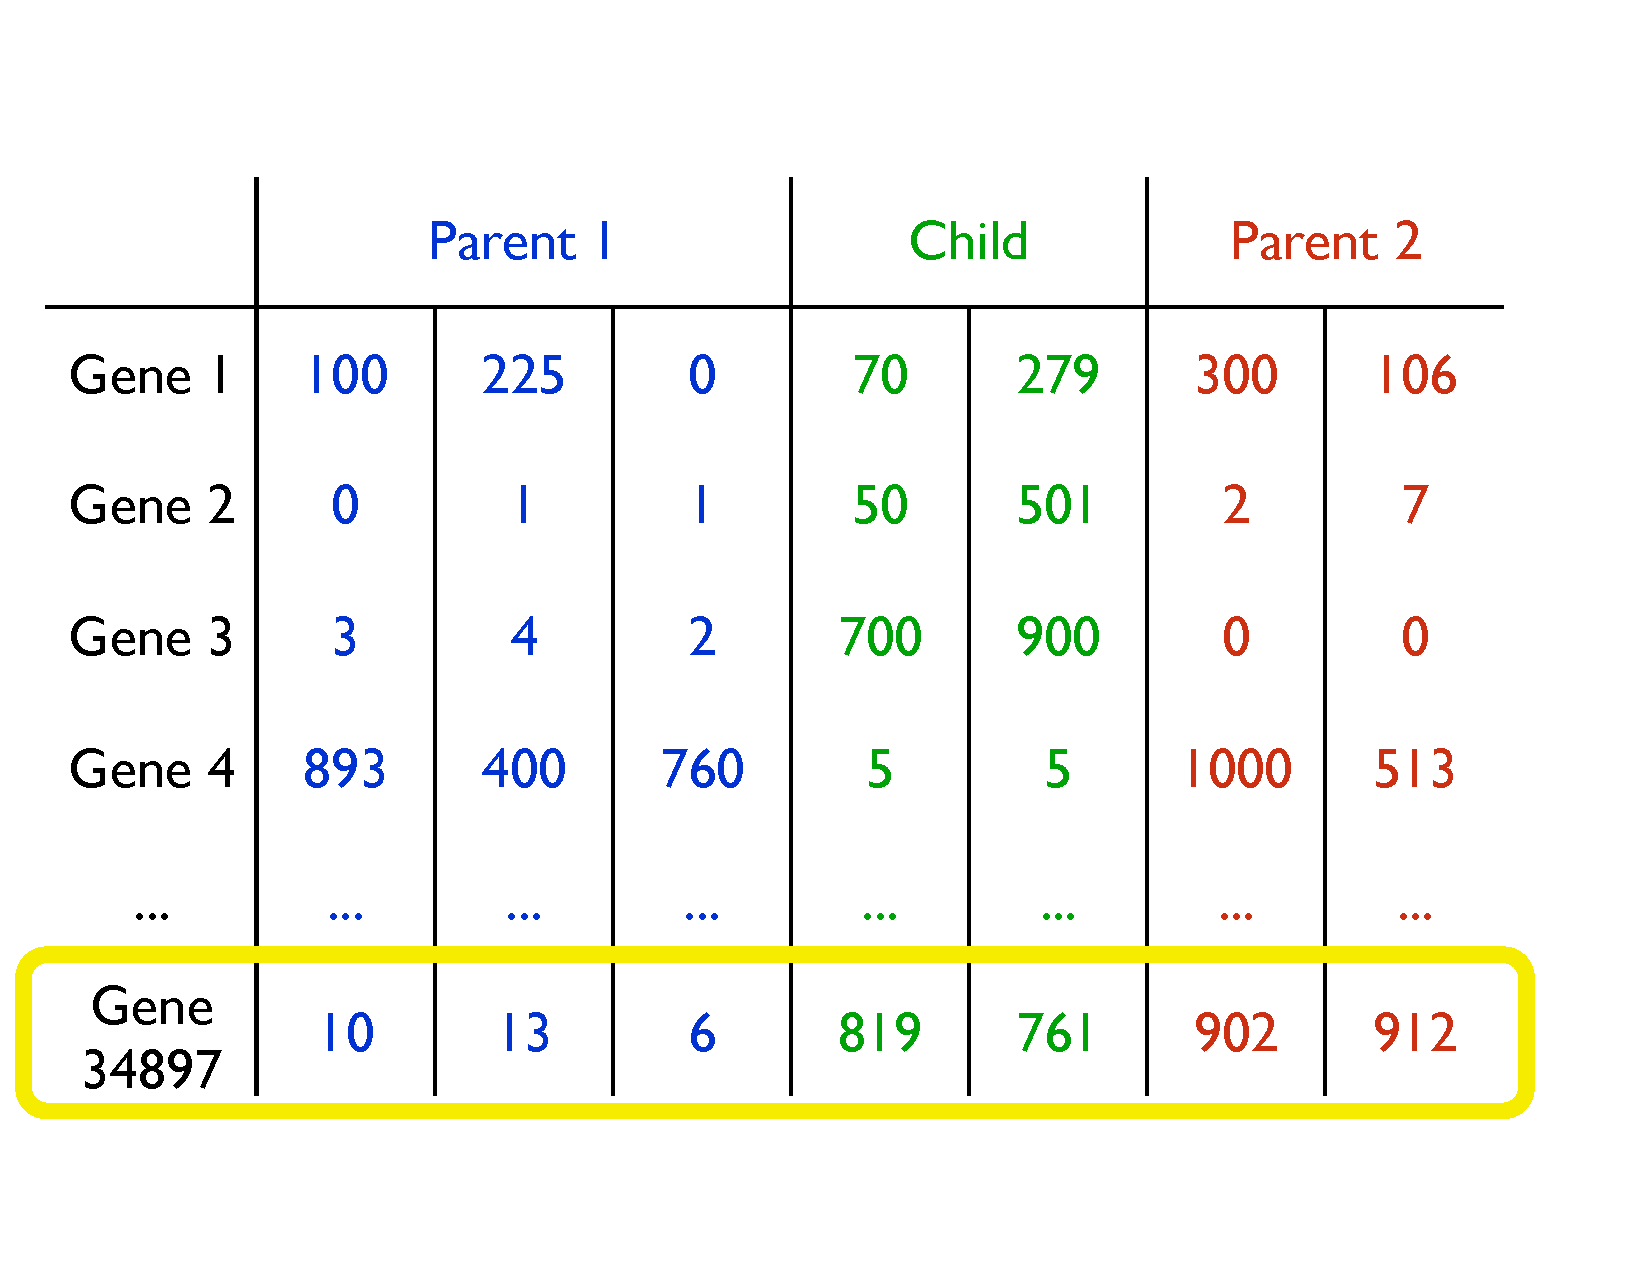
\includegraphics[scale=.35]{fig/mphrnaseq}
\end{center}
\end{frame}


\section{The model}
\setcounter{subsection}{1}

\begin{frame}
\frametitle{The model}

\begin{align*}
& \scriptsize \mu(n, \phi_g, \alpha_g, \delta_g) = \begin{cases}
\phi_g - \alpha_g & \text{ sample $n$ from parent 1} \\
\phi_g + \delta_g & \text{ sample $n$ from child} \\
\phi_g + \alpha_g & \text{ sample $n$ from parent 2} \\
\end{cases} \\ 
&y_{g,n} \stackrel{\text{ind}}{\sim} \text{Poisson}(\exp(c_n + \e_{g, n} + \mu(n, \phi_g, \alpha_g, \delta_g))) \\
&\qquad \uncover<2->{\only<2>{\color{blue}}c_n \stackrel{\text{ind}}{\sim} \text{N}(0, \sigma_c^2)} \\
& \qquad \qquad \uncover<4->{\only<4>{\color{blue}}\sigma_c \stackrel{\text{}}{\sim} \text{U}(0, \sigma_{c0})} \\
& \qquad \uncover<3->{\only<3>{\color{blue}}\e_{g, n} \stackrel{\text{ind}}{\sim} \text{N}(0, \eta_g^2)} \\
& \qquad \qquad \uncover<5->{\only<5>{\color{blue}}\eta_g^2 \stackrel{\text{ind}}{\sim} \text{Inv-Gamma}\left (\left . \text{shape} = \frac{d}{2} \right ., \ \text{rate} =  \frac{d \cdot \tau^2}{2} \right)} \\
& \qquad \qquad \qquad \uncover<6->{\only<6>{\color{blue}} d \stackrel{\text{}}{\sim} \text{U}(0, d_0)} \\
& \qquad \qquad \qquad \uncover<7->{\only<7>{\color{blue}} \tau^2 \stackrel{\text{}}{\sim} \text{Gamma}(\text{shape} = a_\tau, \text{rate} = b_\tau)} \\
\end{align*}
\end{frame}


\begin{frame}
\frametitle{The model} \tiny

\begin{align*}
&\scriptsize \mu(n, \phi_g, \alpha_g, \delta_g) = \begin{cases}
\phi_g - \alpha_g & \text{ sample $n$ from parent 1} \\
\phi_g + \delta_g & \text{ sample $n$ from child} \\
\phi_g + \alpha_g & \text{ sample $n$ from parent 2} \\
\end{cases} \\ 
&{\scriptsize y_{g,n} \stackrel{\text{ind}}{\sim} \text{Poisson}(\exp(c_n + \e_{g, n} + \mu(n, \phi_g, \alpha_g, \delta_g)))} \\
& \qquad \uncover<3->{\only<3>{\color{blue}}\phi_g \stackrel{\text{ind}}{\sim} \text{N}( \theta_\phi, \sigma_\phi^2)} \\
& \qquad \qquad \uncover<6->{\only<6>{\color{blue}}\theta_\phi \stackrel{\text{}}{\sim} \text{N}( 0, \gamma_{\phi }^2)} \\
& \qquad \qquad \uncover<9->{\only<9>{\color{blue}}\sigma_\phi \stackrel{\text{}}{\sim} \text{U}( 0, \sigma_{\phi 0})} \\
& \qquad \uncover<4->{\only<4>{\color{blue}} \alpha_g \stackrel{\text{ind}}{\sim} (1-I(\alpha_g)) \cdot \pi_\alpha + I(\alpha_g) \cdot (1- \pi_\alpha) \cdot \text{N}(\alpha_g \mid  \theta_\alpha, \sigma_\alpha^2)} \\
& \qquad \qquad \uncover<7->{\only<7>{\color{blue}}\theta_\alpha \stackrel{\text{}}{\sim} \text{N}(0, \ \gamma_{\alpha}^2)} \\
& \qquad \qquad \uncover<10->{\only<10>{\color{blue}}\sigma_\alpha \stackrel{\text{}}{\sim} \text{U}( 0, \ \sigma_{\alpha 0})} \\
& \qquad \qquad \uncover<12->{\only<12>{\color{blue}}\pi_\alpha \stackrel{\text{}}{\sim} \text{Beta}( a_{\alpha}, \ b_{\alpha})} \\
& \qquad \uncover<5->{\only<5>{\color{blue}}\delta_g \stackrel{\text{ind}}{\sim} (1-I(\delta_g)) \cdot \pi_\delta + I(\delta_g) \cdot (1- \pi_\delta) \cdot \text{N}(\delta_g \mid  \theta_\delta, \sigma_\delta^2) \\
& \qquad \qquad \uncover<8->{\only<8>{\color{blue}}\theta_\delta \stackrel{\text{}}{\sim} \text{N}( 0, \gamma_{\delta}^2)}} \\
& \qquad \qquad \uncover<11->{\only<11>{\color{blue}}\sigma_\delta \stackrel{\text{}}{\sim} \text{U}( 0, \sigma_{\delta 0})} \\
& \qquad \qquad \uncover<13->{\only<13>{\color{blue}}\pi_\delta \stackrel{\text{}}{\sim} \text{Beta}( a_{\delta}, b_{\delta})} \\
\end{align*}

\end{frame}


\section{The Gibbs sampler}

\subsection{Gibbs steps}

\begin{frame}
\frametitle{Partition parameters by conditional independence.}
\begin{center}
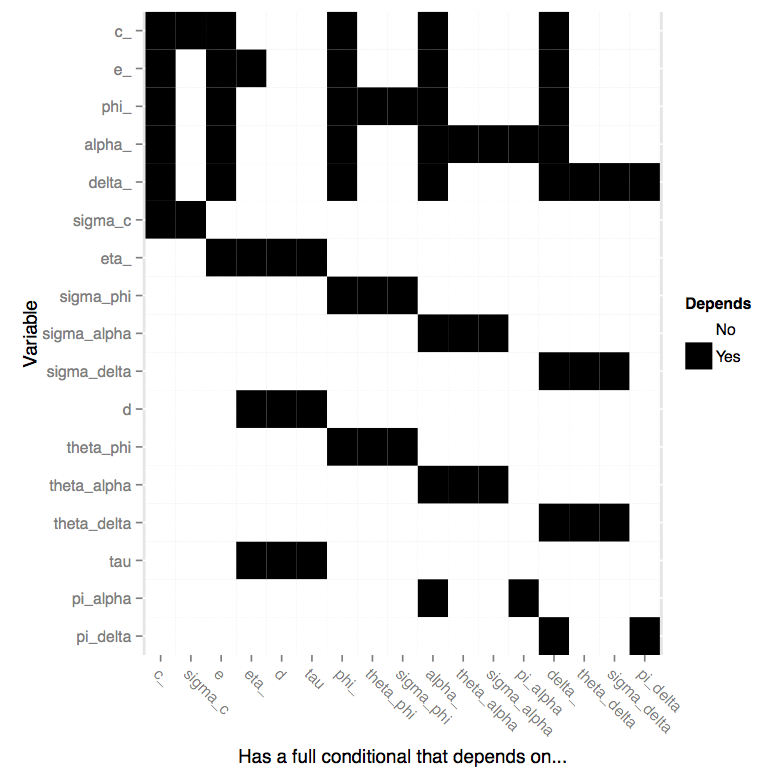
\includegraphics[scale=.25]{fig/depend.png}
\end{center}
\end{frame}

\begin{frame}
\frametitle{Use these partitions as Gibbs steps.} \small

\begin{align*}
y_{g,n} \stackrel{\text{ind}}{\sim} \text{Poisson}( \exp(c_n + \e_{g, n} + \mu(n, \phi_g, \alpha_g, \delta_g)))
\end{align*}

\begin{itemize}
\item From the appropriate full conditional distributions, sample the following:
\end{itemize}


\begin{enumerate}
\item $c_1, \ \ldots, \ c_N$
\pause \item $\tau, \ \pi_\alpha, \ \pi_\delta$
\pause \item $d, \ \theta_\phi, \ \theta_\alpha, \ \theta_\delta$
\pause \item $\sigma_c, \ \sigma_\phi, \ \sigma_\alpha, \ \sigma_\delta, \ \eta_1^2, \ \ldots, \ \eta_G^2$
\pause \item $\e_{1, 1}, \ \e_{1, 2}, \ \ldots, \ \e_{1, N}, \ \e_{2, N}, \ \ldots, \ \e_{G, N}$
\pause \item $\phi_1, \ \ldots, \ \phi_G$
\pause \item $\alpha_1, \ \ldots, \ \alpha_G$
\pause \item $\delta_1, \ \ldots, \ \delta_G$
\end{enumerate}
\begin{itemize}
\item and then repeat.
\end{itemize}
\end{frame}

\subsection{Estimated heterosis probabilities}

\begin{frame}
\frametitle{Estimated heterosis probabilities} \small
\begin{align*}
& \scriptsize \mu(n, \phi_g, \alpha_g, \delta_g) = \begin{cases}
\phi_g - \alpha_g & \text{ sample $n$ from parent 1} \\
\phi_g + \delta_g & \text{ sample $n$ from child} \\
\phi_g + \alpha_g & \text{ sample $n$ from parent 2} \\
\end{cases} \\ \\
&{\scriptsize y_{g,n} \stackrel{\text{ind}}{\sim} \text{Poisson}( \exp(c_n + \e_{g, n} + \mu(n, \phi_g, \alpha_g, \delta_g)))} \\ 
\uncover<2->{\intertext{Consider one chain with $M$ iterations.}}
&\uncover<3->{P(\text{high-parent heterosis in gene } g) \approx \frac{1}{M} \sum_{i = 1}^M I(\delta_g^{(i)} > |\alpha_g^{(i)}|)} \\
&\uncover<4->{P(\text{low-parent heterosis in gene } g \text{ }) \approx \frac{1}{M} \sum_{i = 1}^M I(\delta_g^{(i)} < -|\alpha_g^{(i)}|)} \\
&\uncover<5->{P(\text{mid-parent heterosis in gene } g \text{ }) \approx \frac{1}{M} \sum_{i = 1}^M I(\delta_g^{(i)} \ne 0)}
\end{align*}
\end{frame}


\subsection{GPU parallelism}

\begin{frame}
\frametitle{Tons of opportunity for GPU parallelism across genes!}
\begin{align*}
y_{g,n} \stackrel{\text{ind}}{\sim} \text{Poisson}( \exp(c_n + \e_{g, n} + \mu(n, \phi_g, \alpha_g, \delta_g)))
\end{align*}

\begin{itemize}
\item Sample in parallel:
\begin{itemize}
\pause \item $\phi_g$'s
\pause \item $\alpha_g$'s
\pause \item $\delta_g$'s
\pause \item $\e_{g, n}$'s 
\pause \item $\eta_{g}$'s 
\end{itemize}
\end{itemize}
\end{frame}



% INSERT CUDA SLIDES HERE


\begin{frame}
\frametitle{Example: $\phi_g$'s} \small
\begin{align*}
&y_{g,n} \stackrel{\text{ind}}{\sim} \text{Poisson}( \exp(c_n + \e_{g, n} + \mu(n, \phi_g, \alpha_g, \delta_g))) \\
& \qquad \uncover<2->{\phi_g \stackrel{\text{ind}}{\sim} \text{N}( \theta_\phi, \sigma_\phi^2)} \\
& \qquad \qquad \uncover<3->{\theta_\phi \stackrel{\text{}}{\sim} \text{N}( 0, \gamma_{\phi }^2)} \\
& \qquad \qquad \uncover<4->{\sigma_\phi \stackrel{\text{}}{\sim} \text{U}( 0, \sigma_{\phi 0})} \\
\end{align*}

\begin{itemize}
\uncover<5->{\item Using parallel random walk Metropolis steps, sample the $\phi_g$'s from their full conditional distributions,}
\end{itemize}

\begin{align*}
\uncover<6->{p(\phi_g \mid} & \uncover<6->{ \cdots) \propto \exp \left (\sum_{n = 1}^N \left [y_{g, n} \cdot \mu(n, \phi_g, \alpha_g, \delta_g) \right . \right .}  \\
&\uncover<6->{\left . \left . \frac{}{}- \exp (c_n + \e_{g, n} + \mu(n, \phi_g, \alpha_g, \delta_g)) \right ] - \frac{(\phi_g - \theta_\phi)^2}{2 \sigma_\phi^2} \right )}
\end{align*}
\end{frame}


\begin{frame}
\frametitle{Tons of opportunity for GPU parallelism across genes!}
\begin{align*}
y_{g,n} \stackrel{\text{ind}}{\sim} \text{Poisson}( \exp(c_n + \e_{g, n} + \mu(n, \phi_g, \alpha_g, \delta_g)))
\end{align*}

\begin{itemize}
\pause \item Use {\color{blue} \bf parallel reductions} to calculate sufficient statistics for:
\begin{itemize}
\pause \item $c_n$'s
\pause \item $\tau$, $d$
\pause \item $\theta_\phi$, $\theta_\alpha$, $\theta_\delta$
\pause \item $\sigma_\phi$, $\sigma_\alpha$, $\sigma_\delta$,  $\sigma_c$ 
\pause \item $\pi_\alpha$, $\pi_\delta$
\end{itemize}
\end{itemize}
\end{frame}











\begin{frame}
\frametitle{Pairwise summation: an example reduction}

\begin{itemize}
\item Let's take the pairwise sum of the vector,

\begin{align*}
(5, 2, -3, 1, 1, 8, 2, 6)
\end{align*}

using 1 block of 4 threads.
\end{itemize}
\end{frame}

\begin{frame}
\frametitle{Pairwise summation: an example reduction}
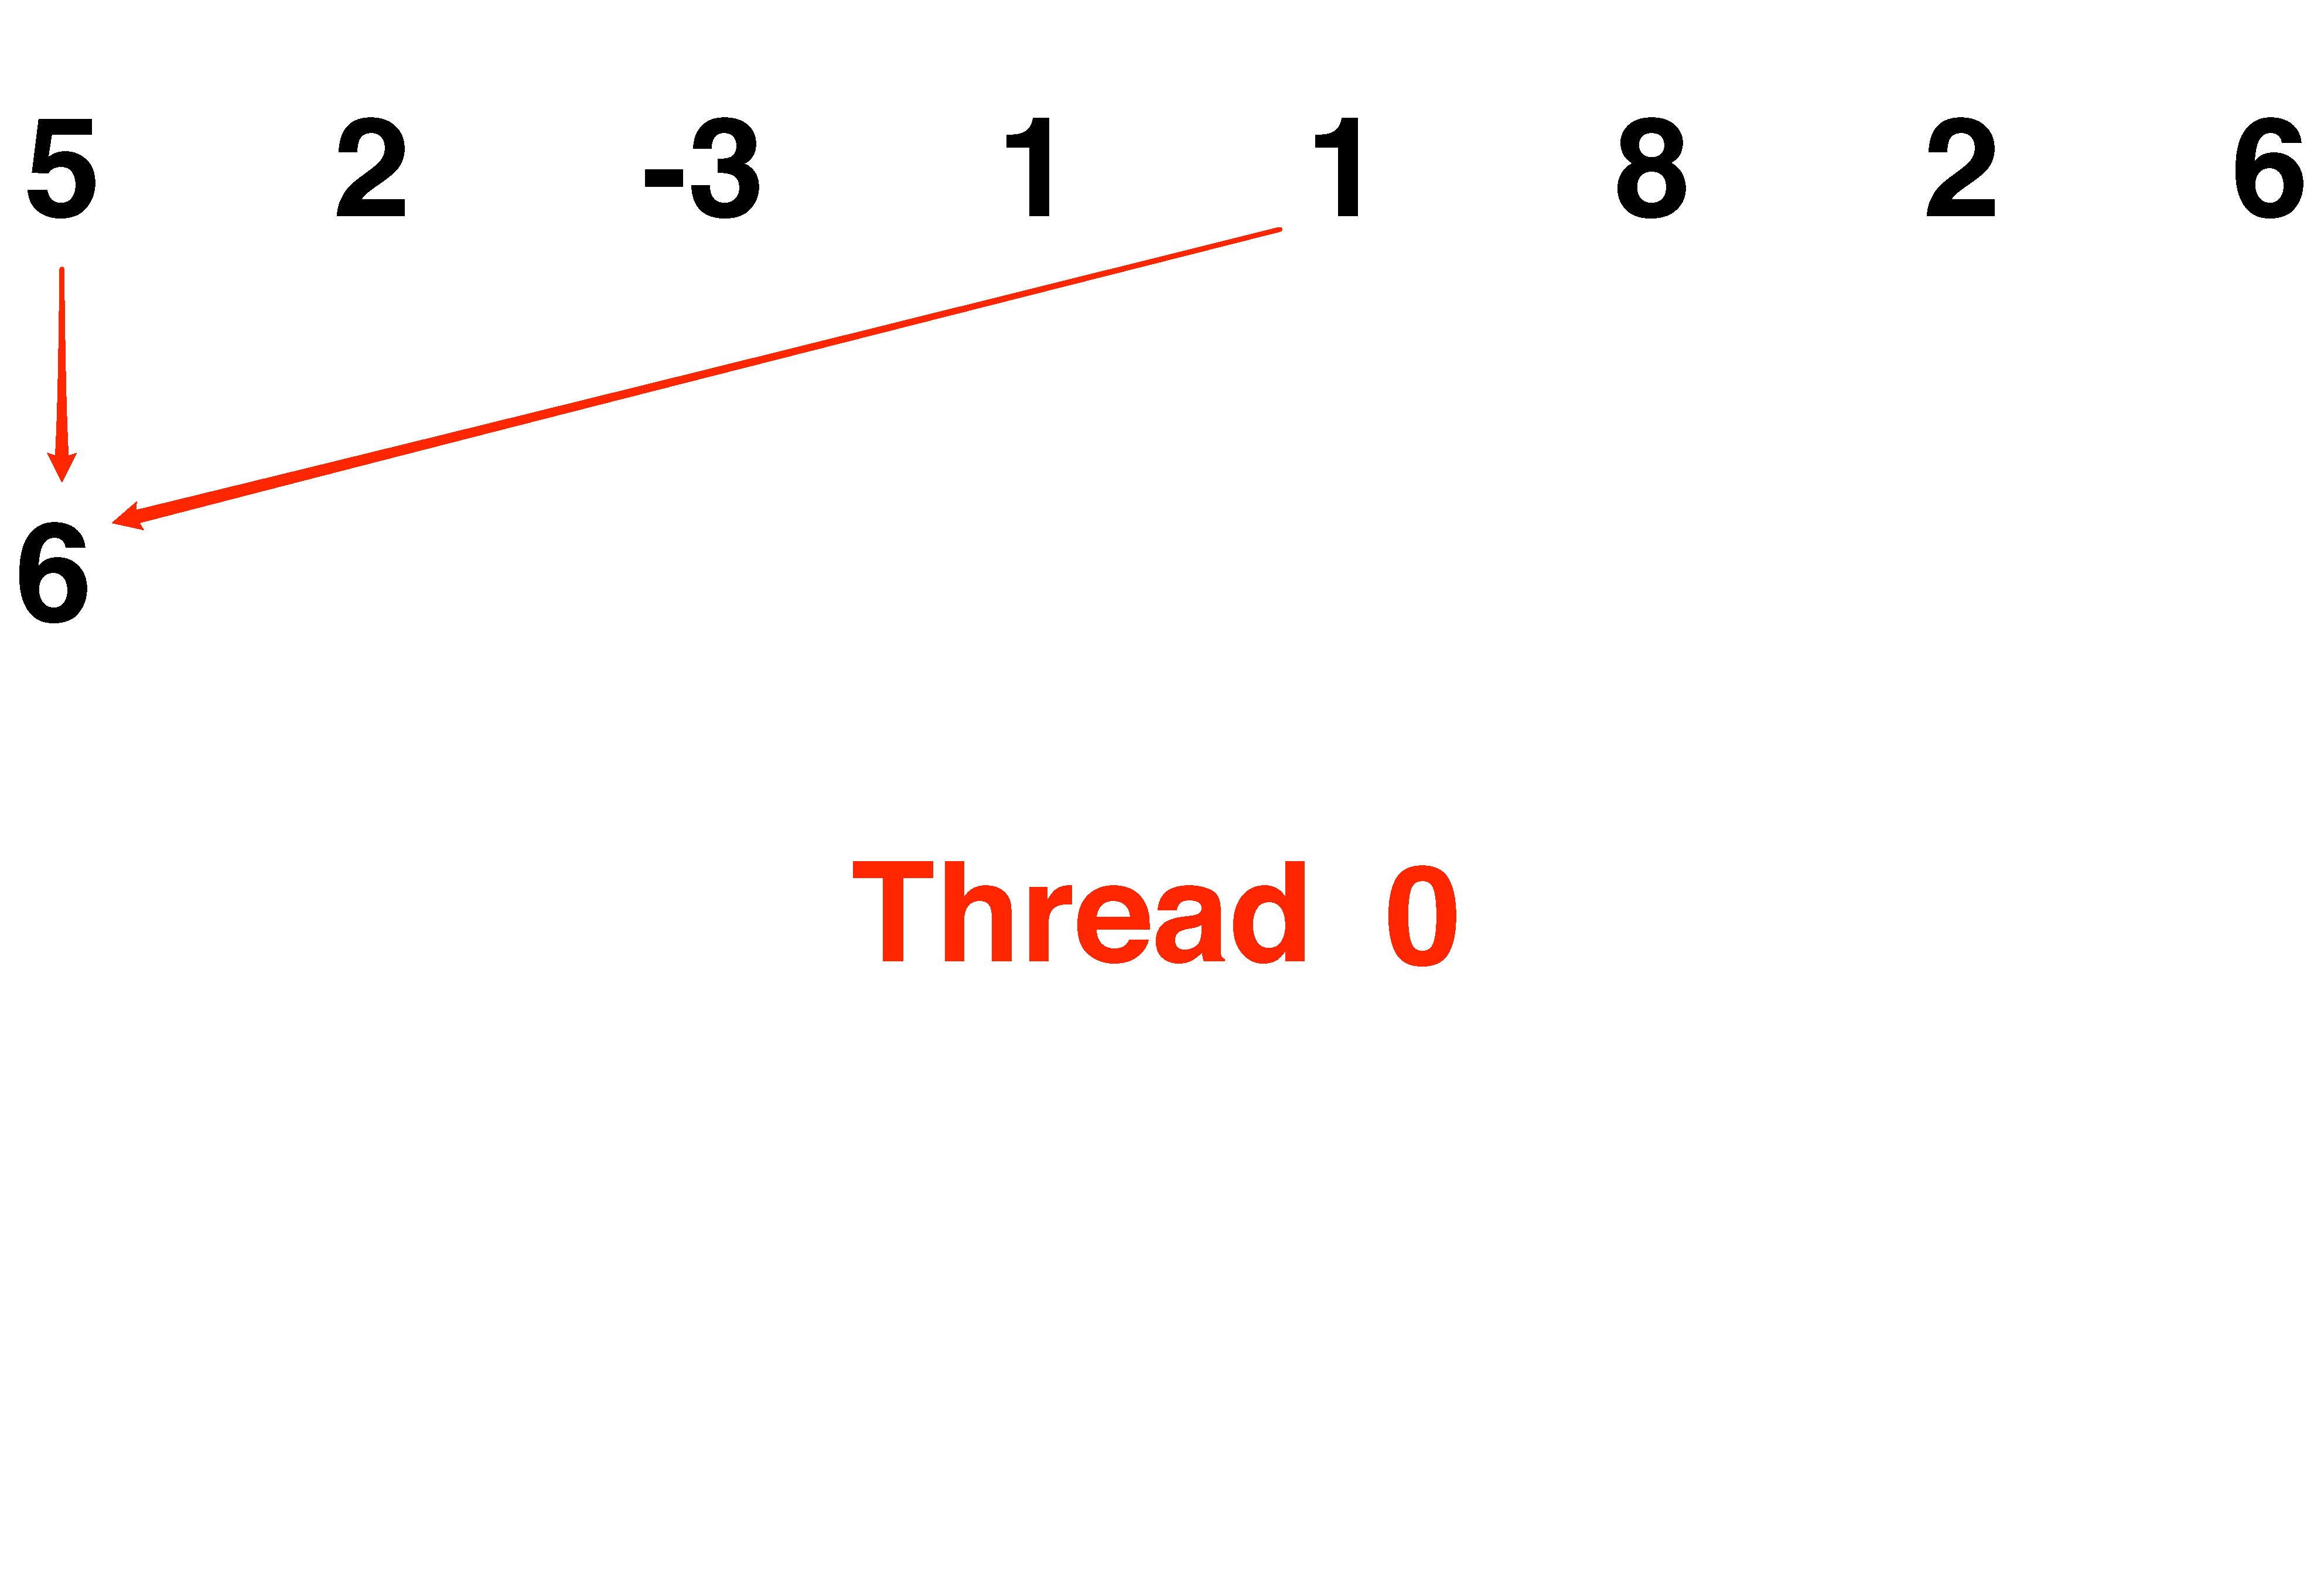
\includegraphics[scale=.15]{fig/psum1.pdf}
\end{frame}

\begin{frame}
\frametitle{Pairwise summation: an example reduction}
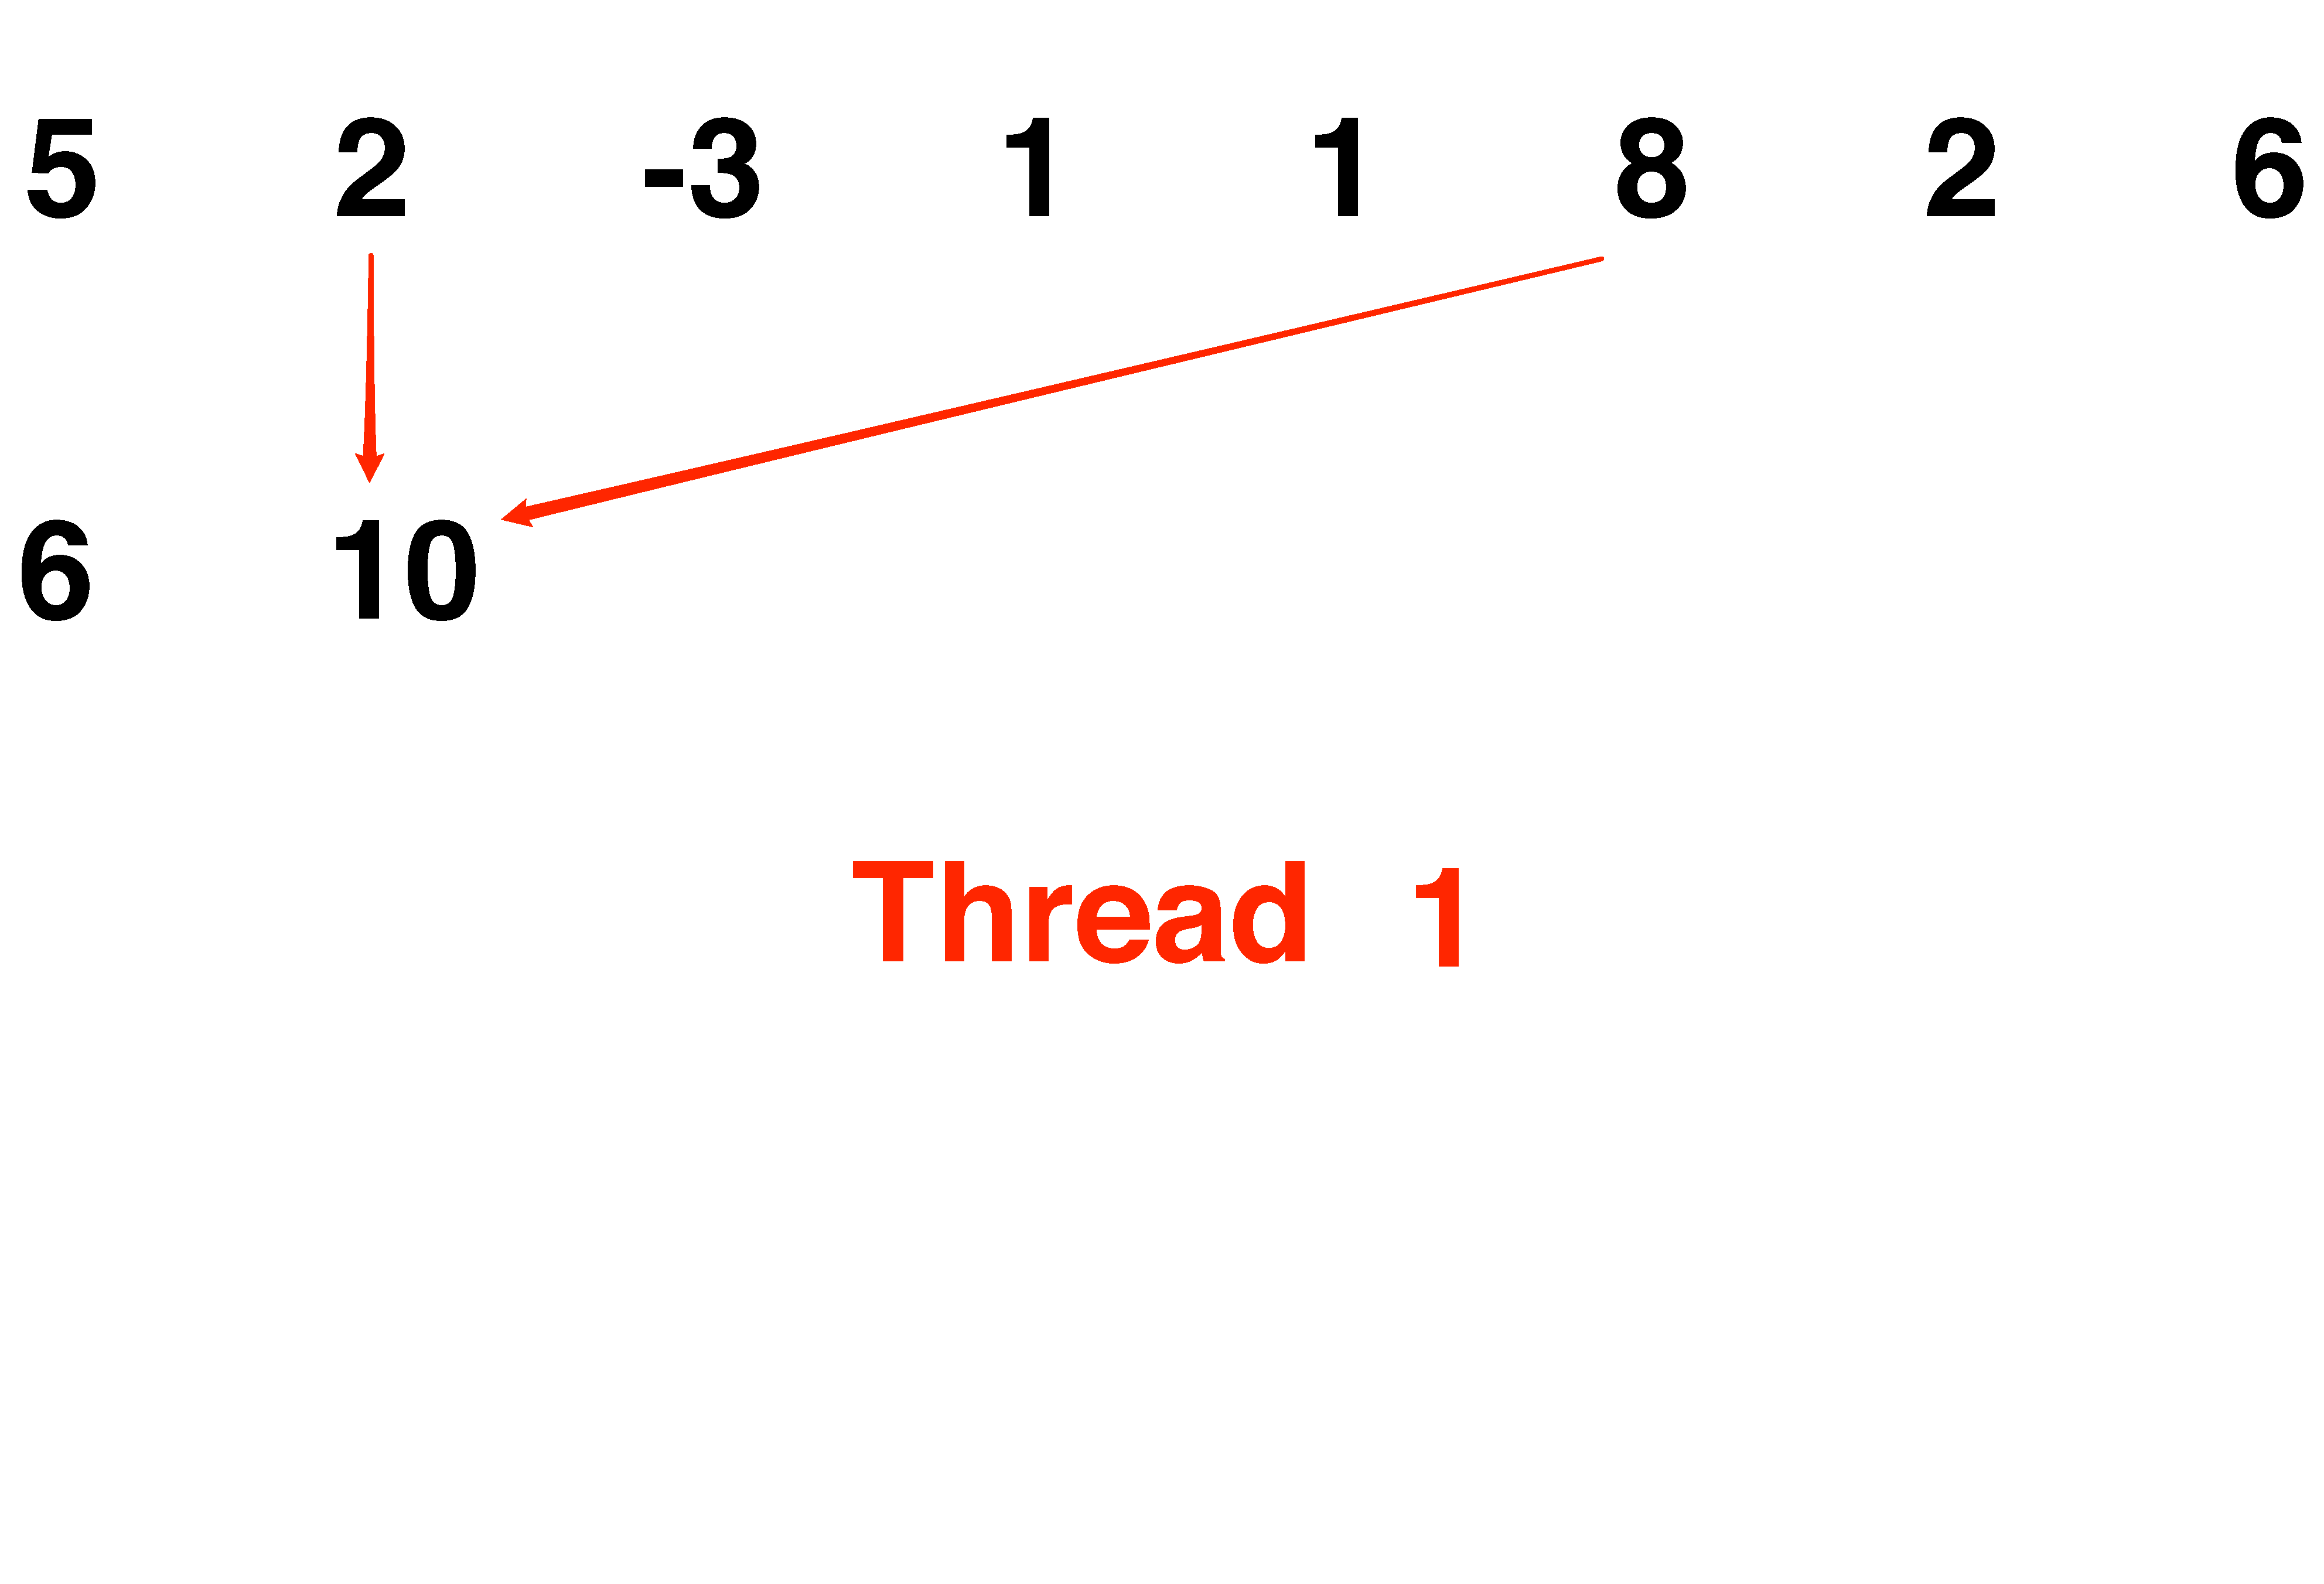
\includegraphics[scale=.15]{fig/psum2.pdf}
\end{frame}

\begin{frame}
\frametitle{Pairwise summation: an example reduction}
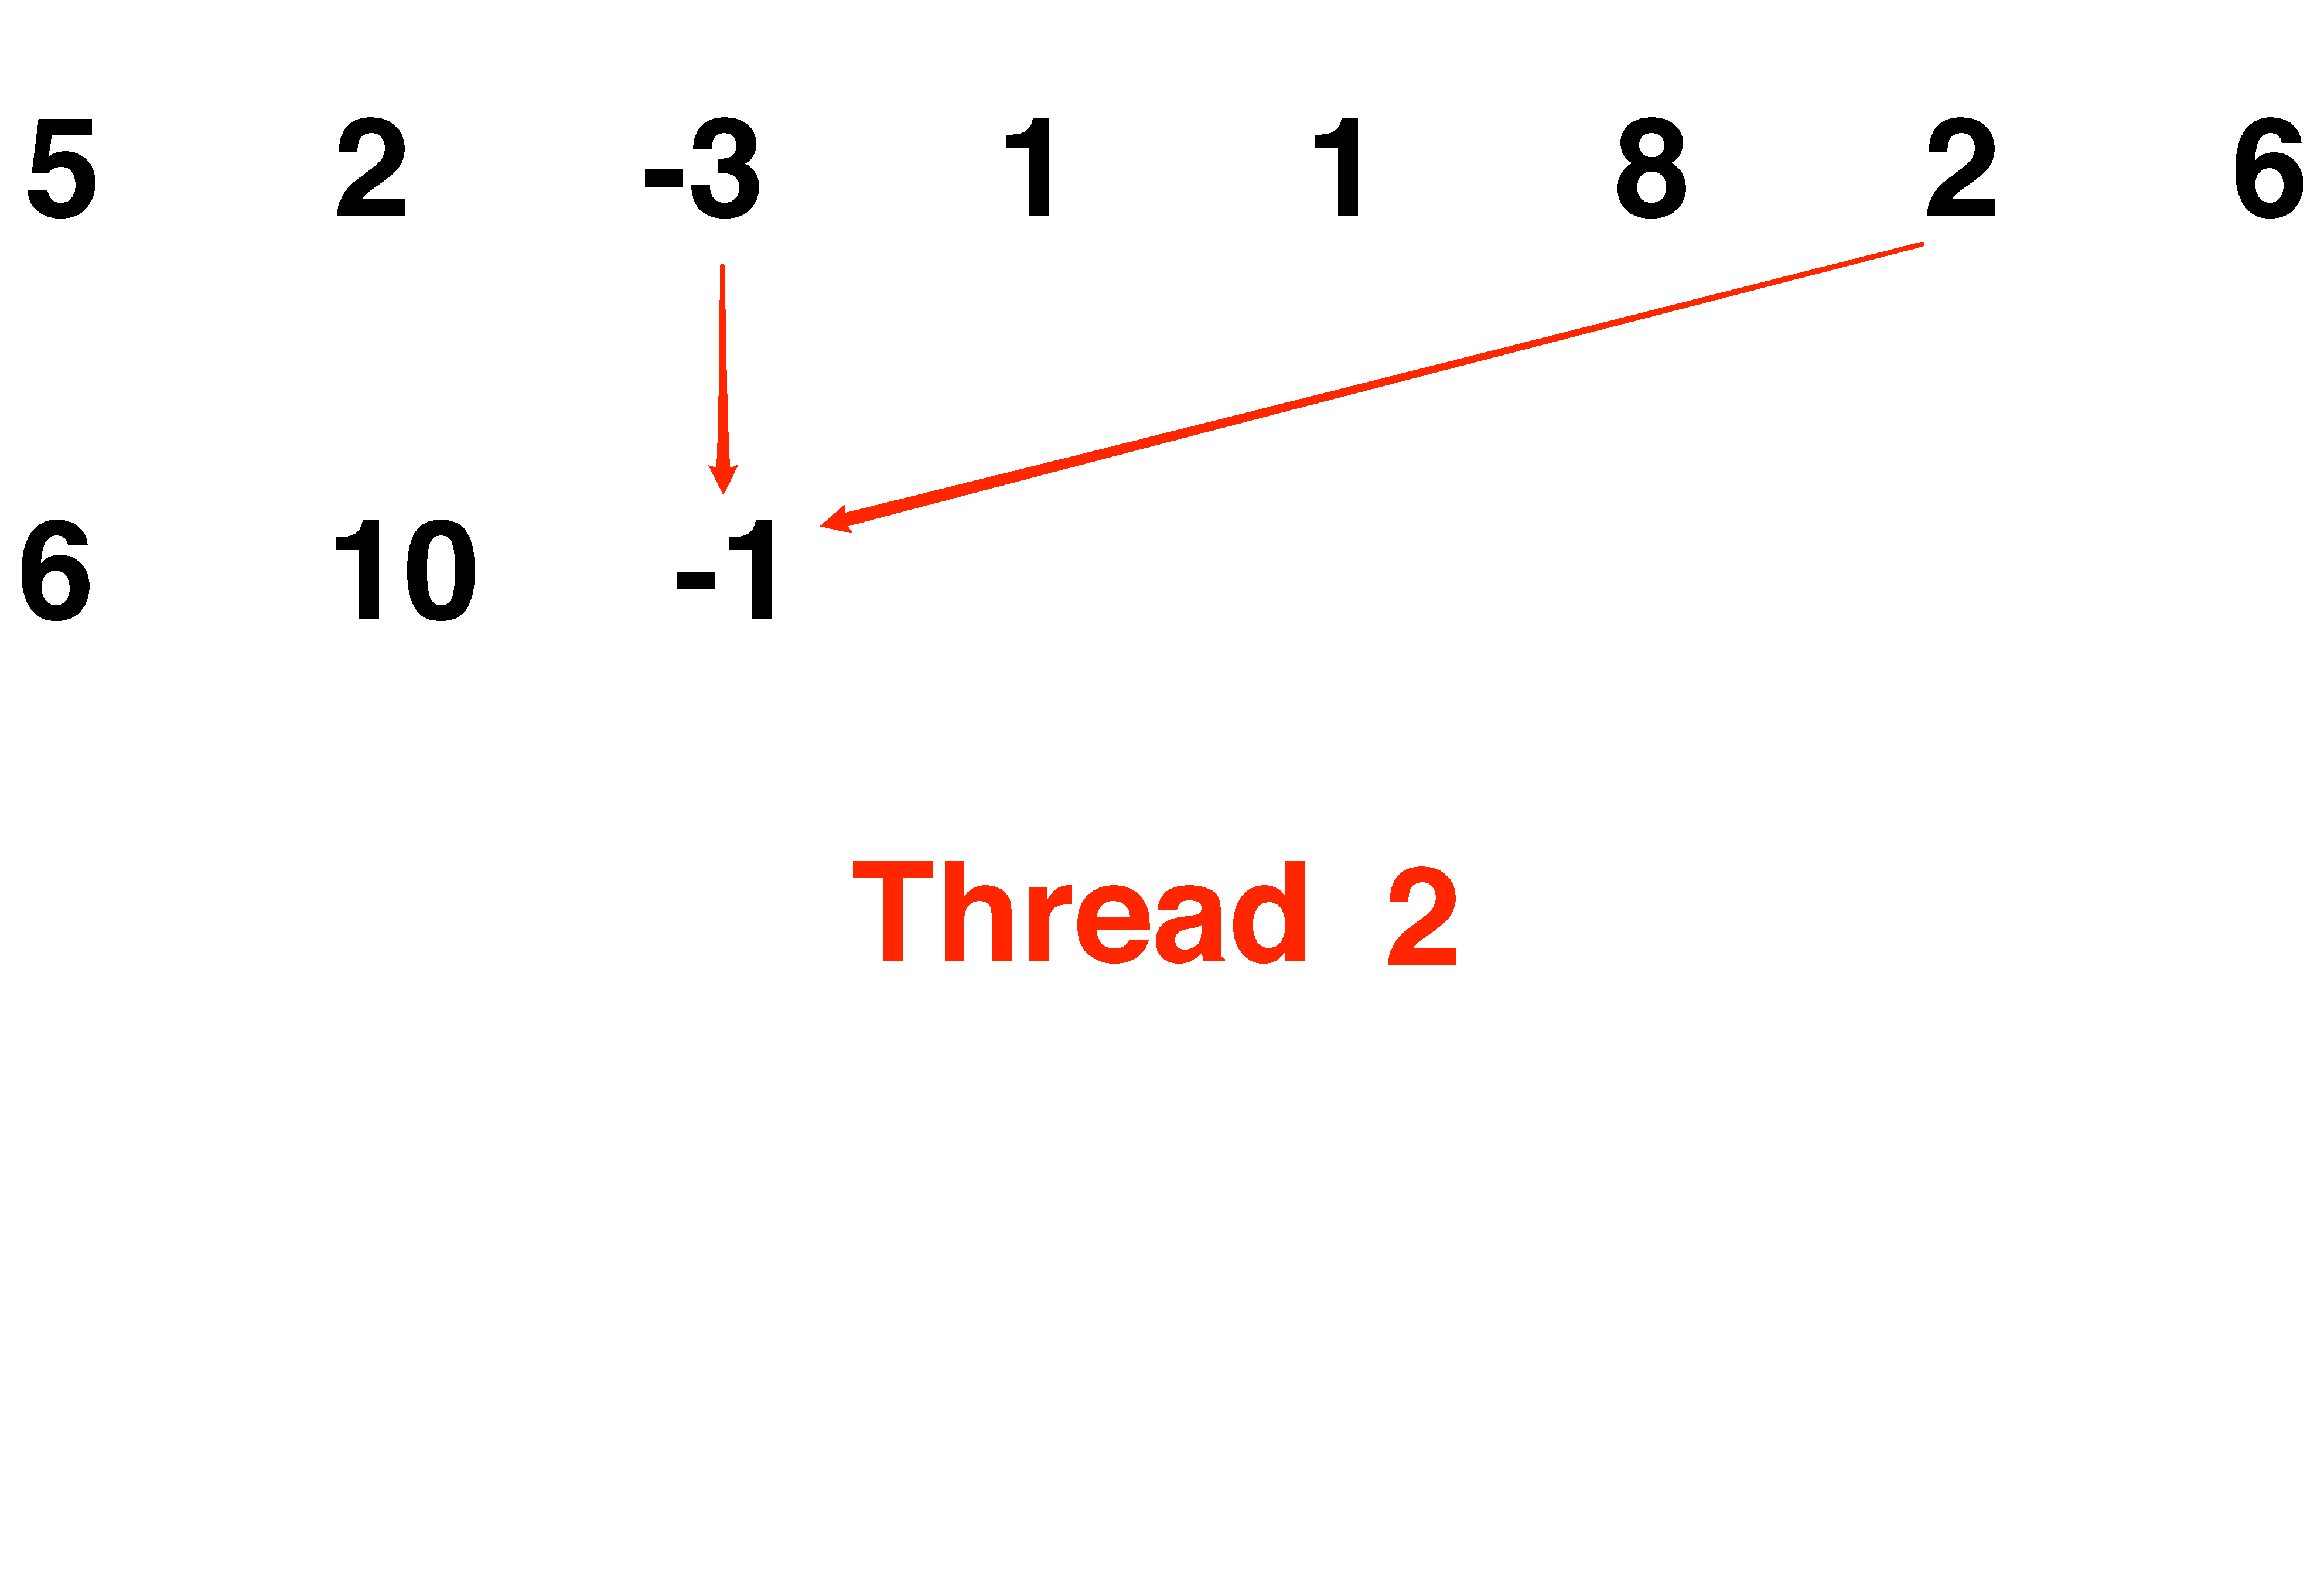
\includegraphics[scale=.15]{fig/psum3.pdf}
\end{frame}
{}
\begin{frame}
\frametitle{Pairwise summation: an example reduction}
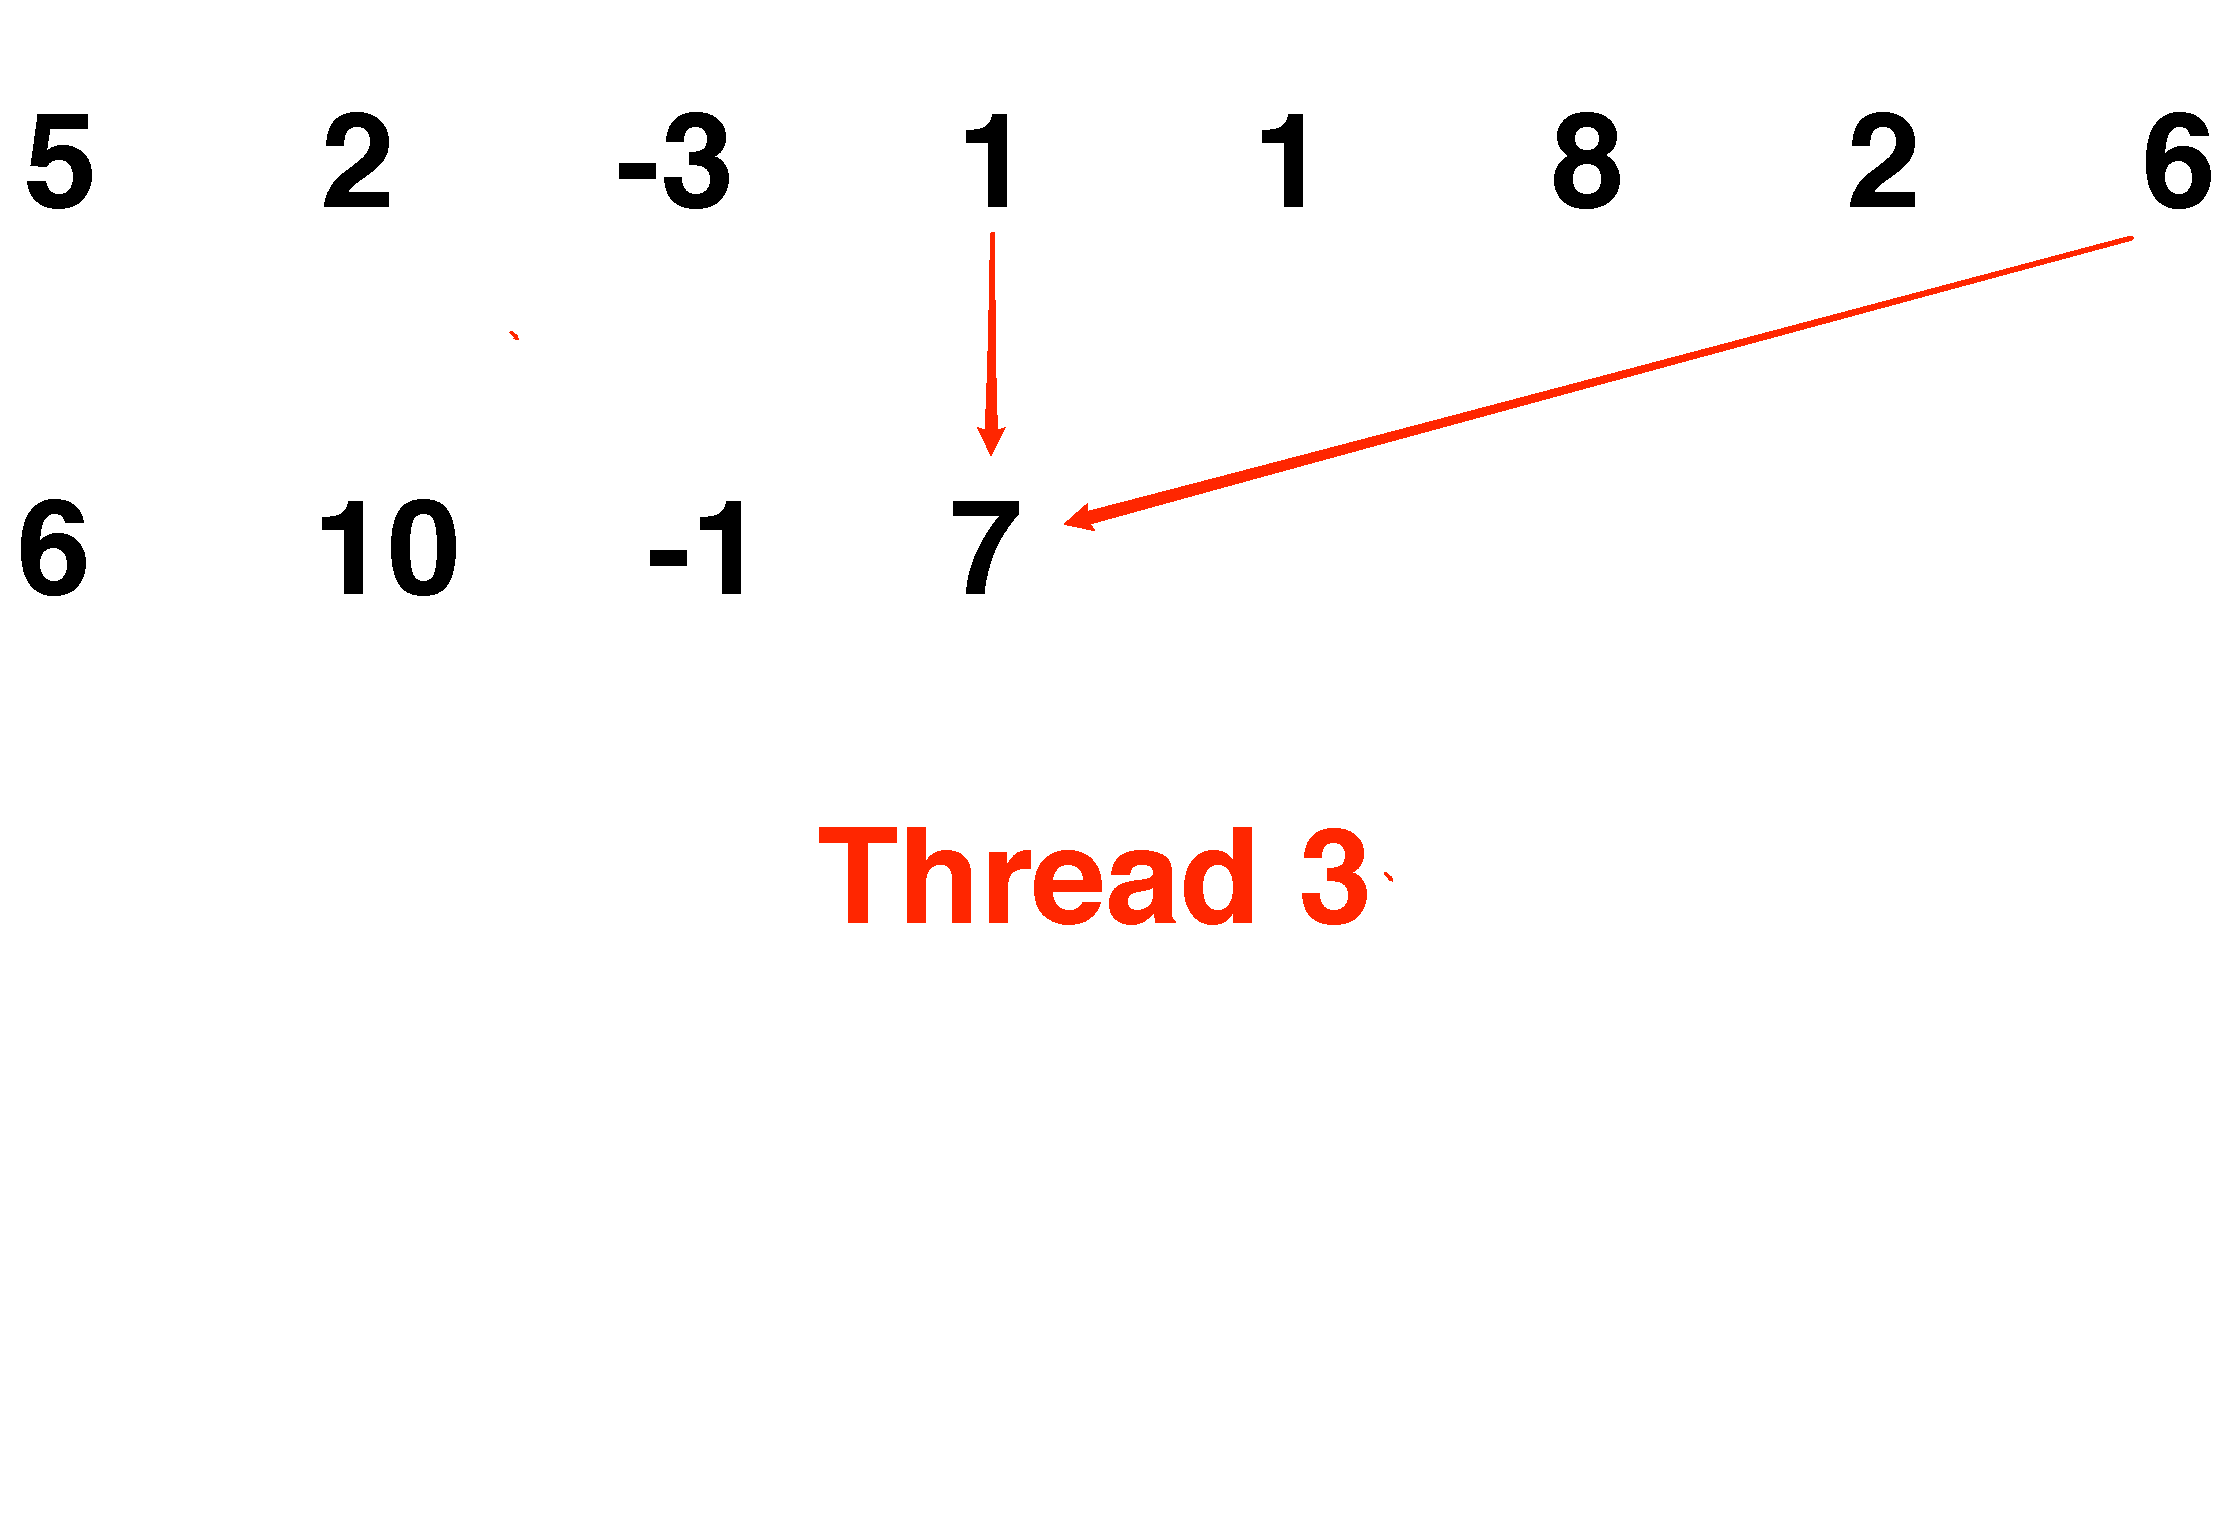
\includegraphics[scale=.25]{fig/psum4.pdf}
\end{frame}

\begin{frame}
\frametitle{Pairwise summation: an example reduction}
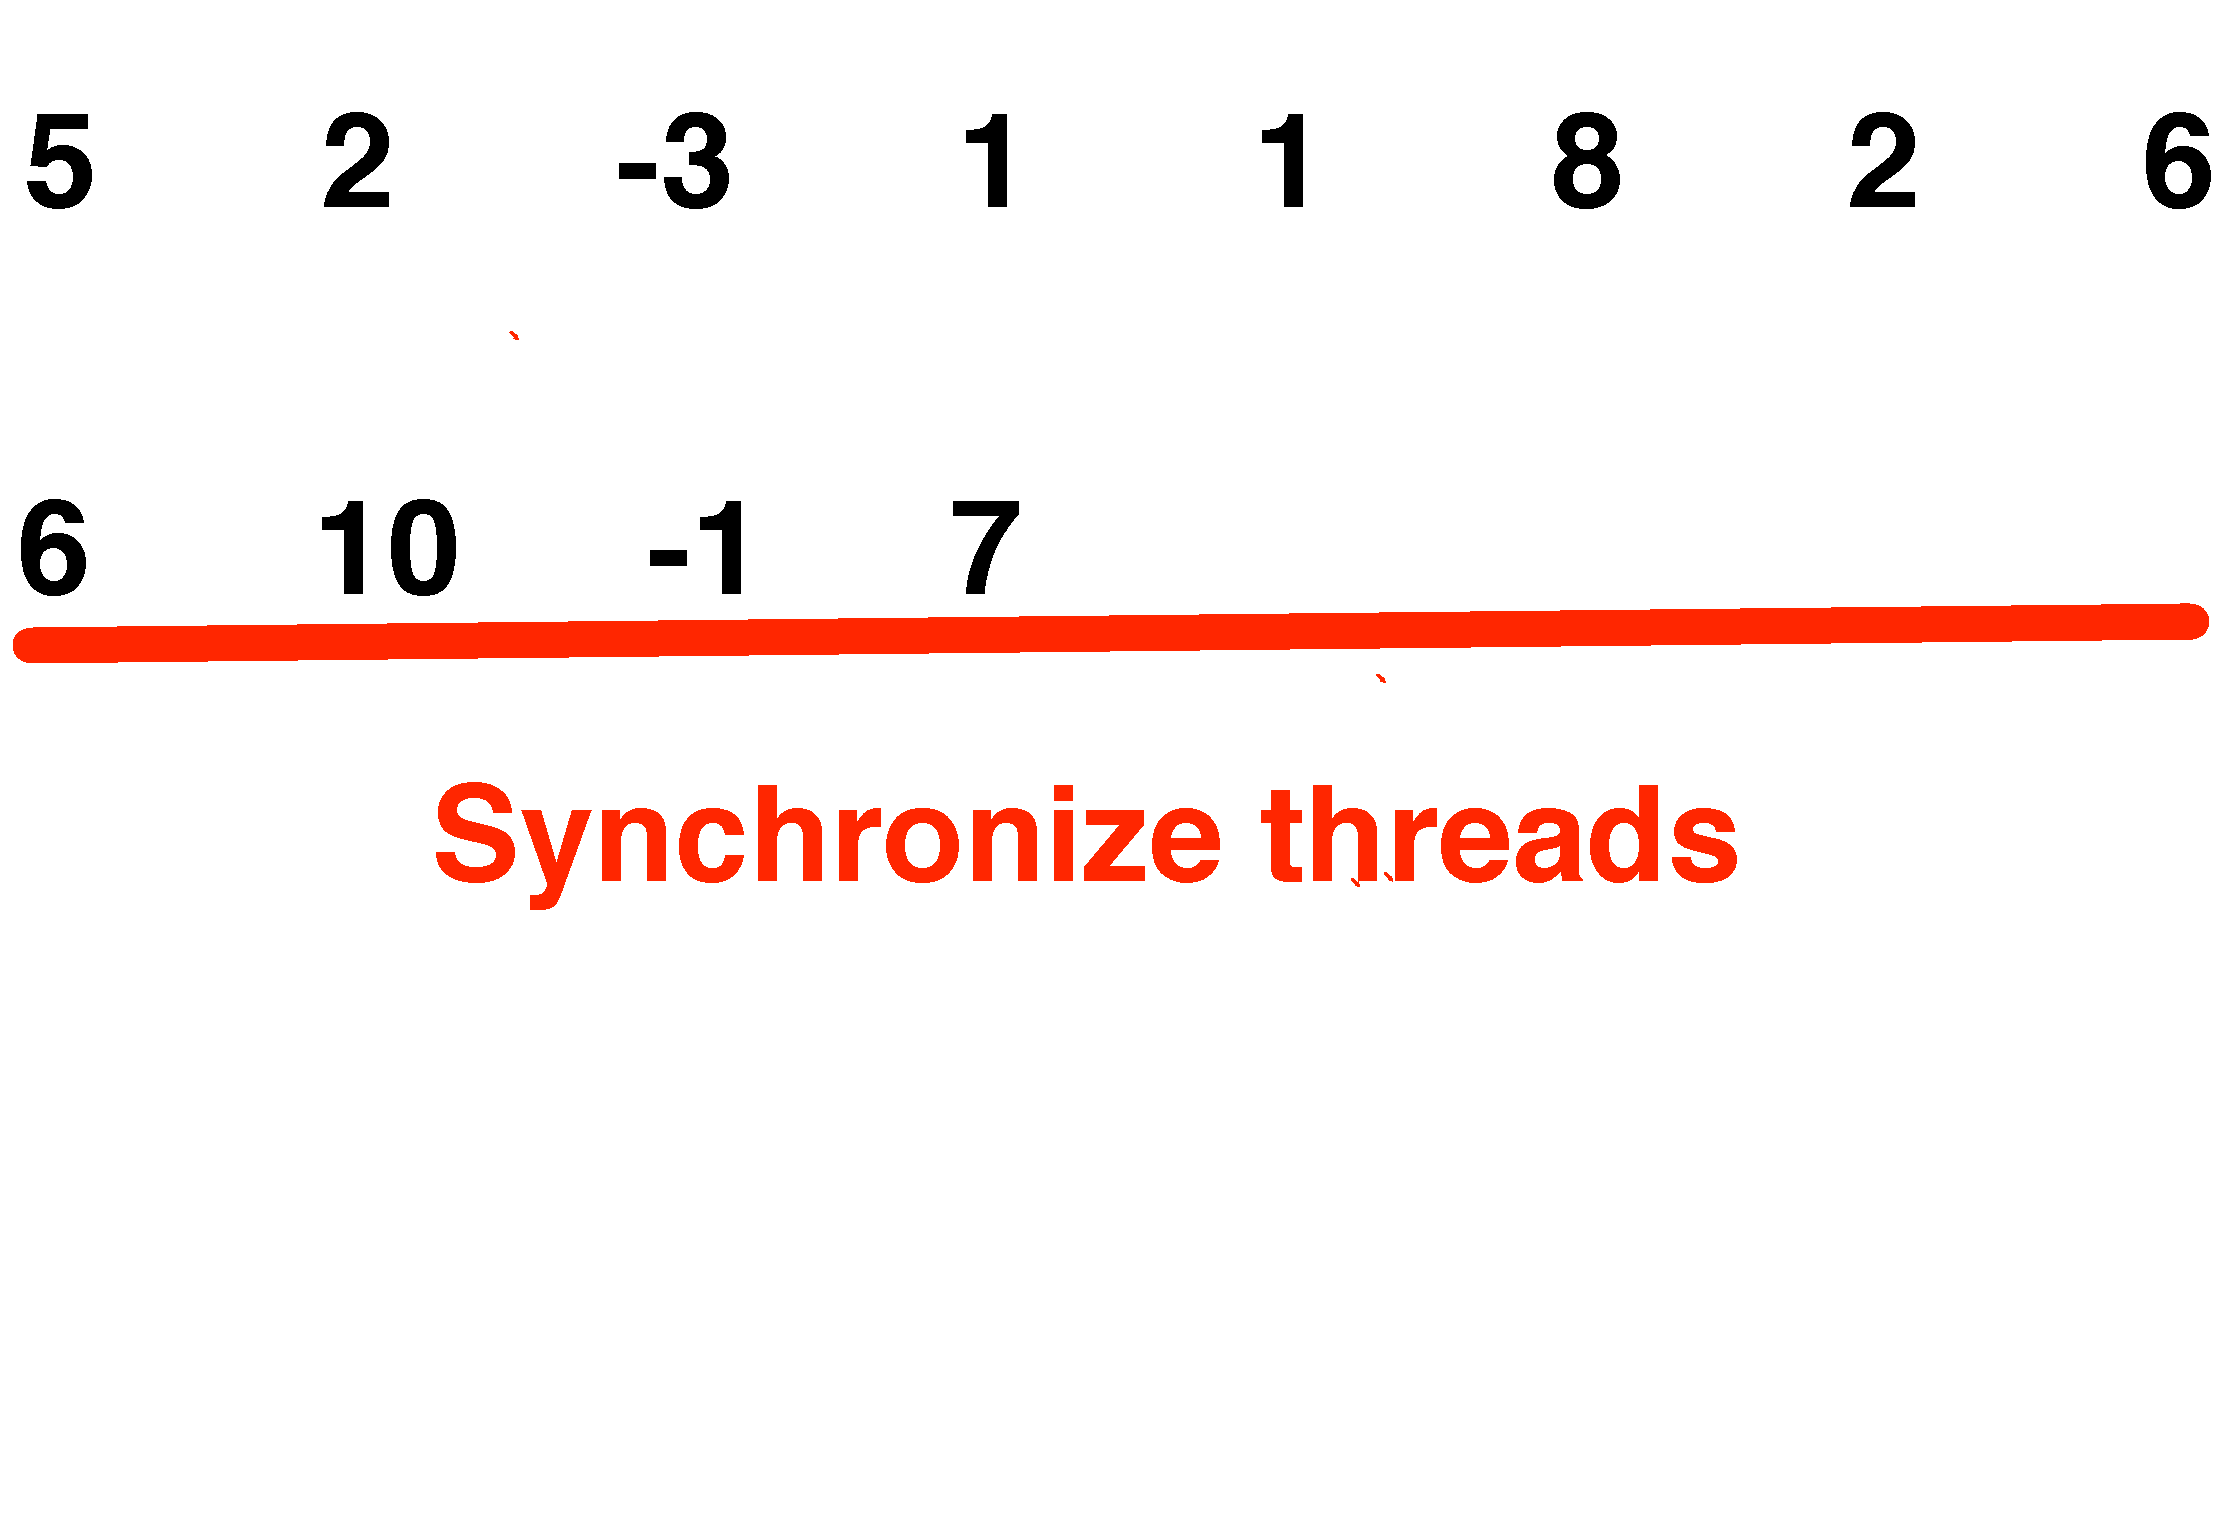
\includegraphics[scale=.25]{fig/psum5.pdf}
\end{frame}


\begin{frame}
\frametitle{Pairwise summation: an example reduction}
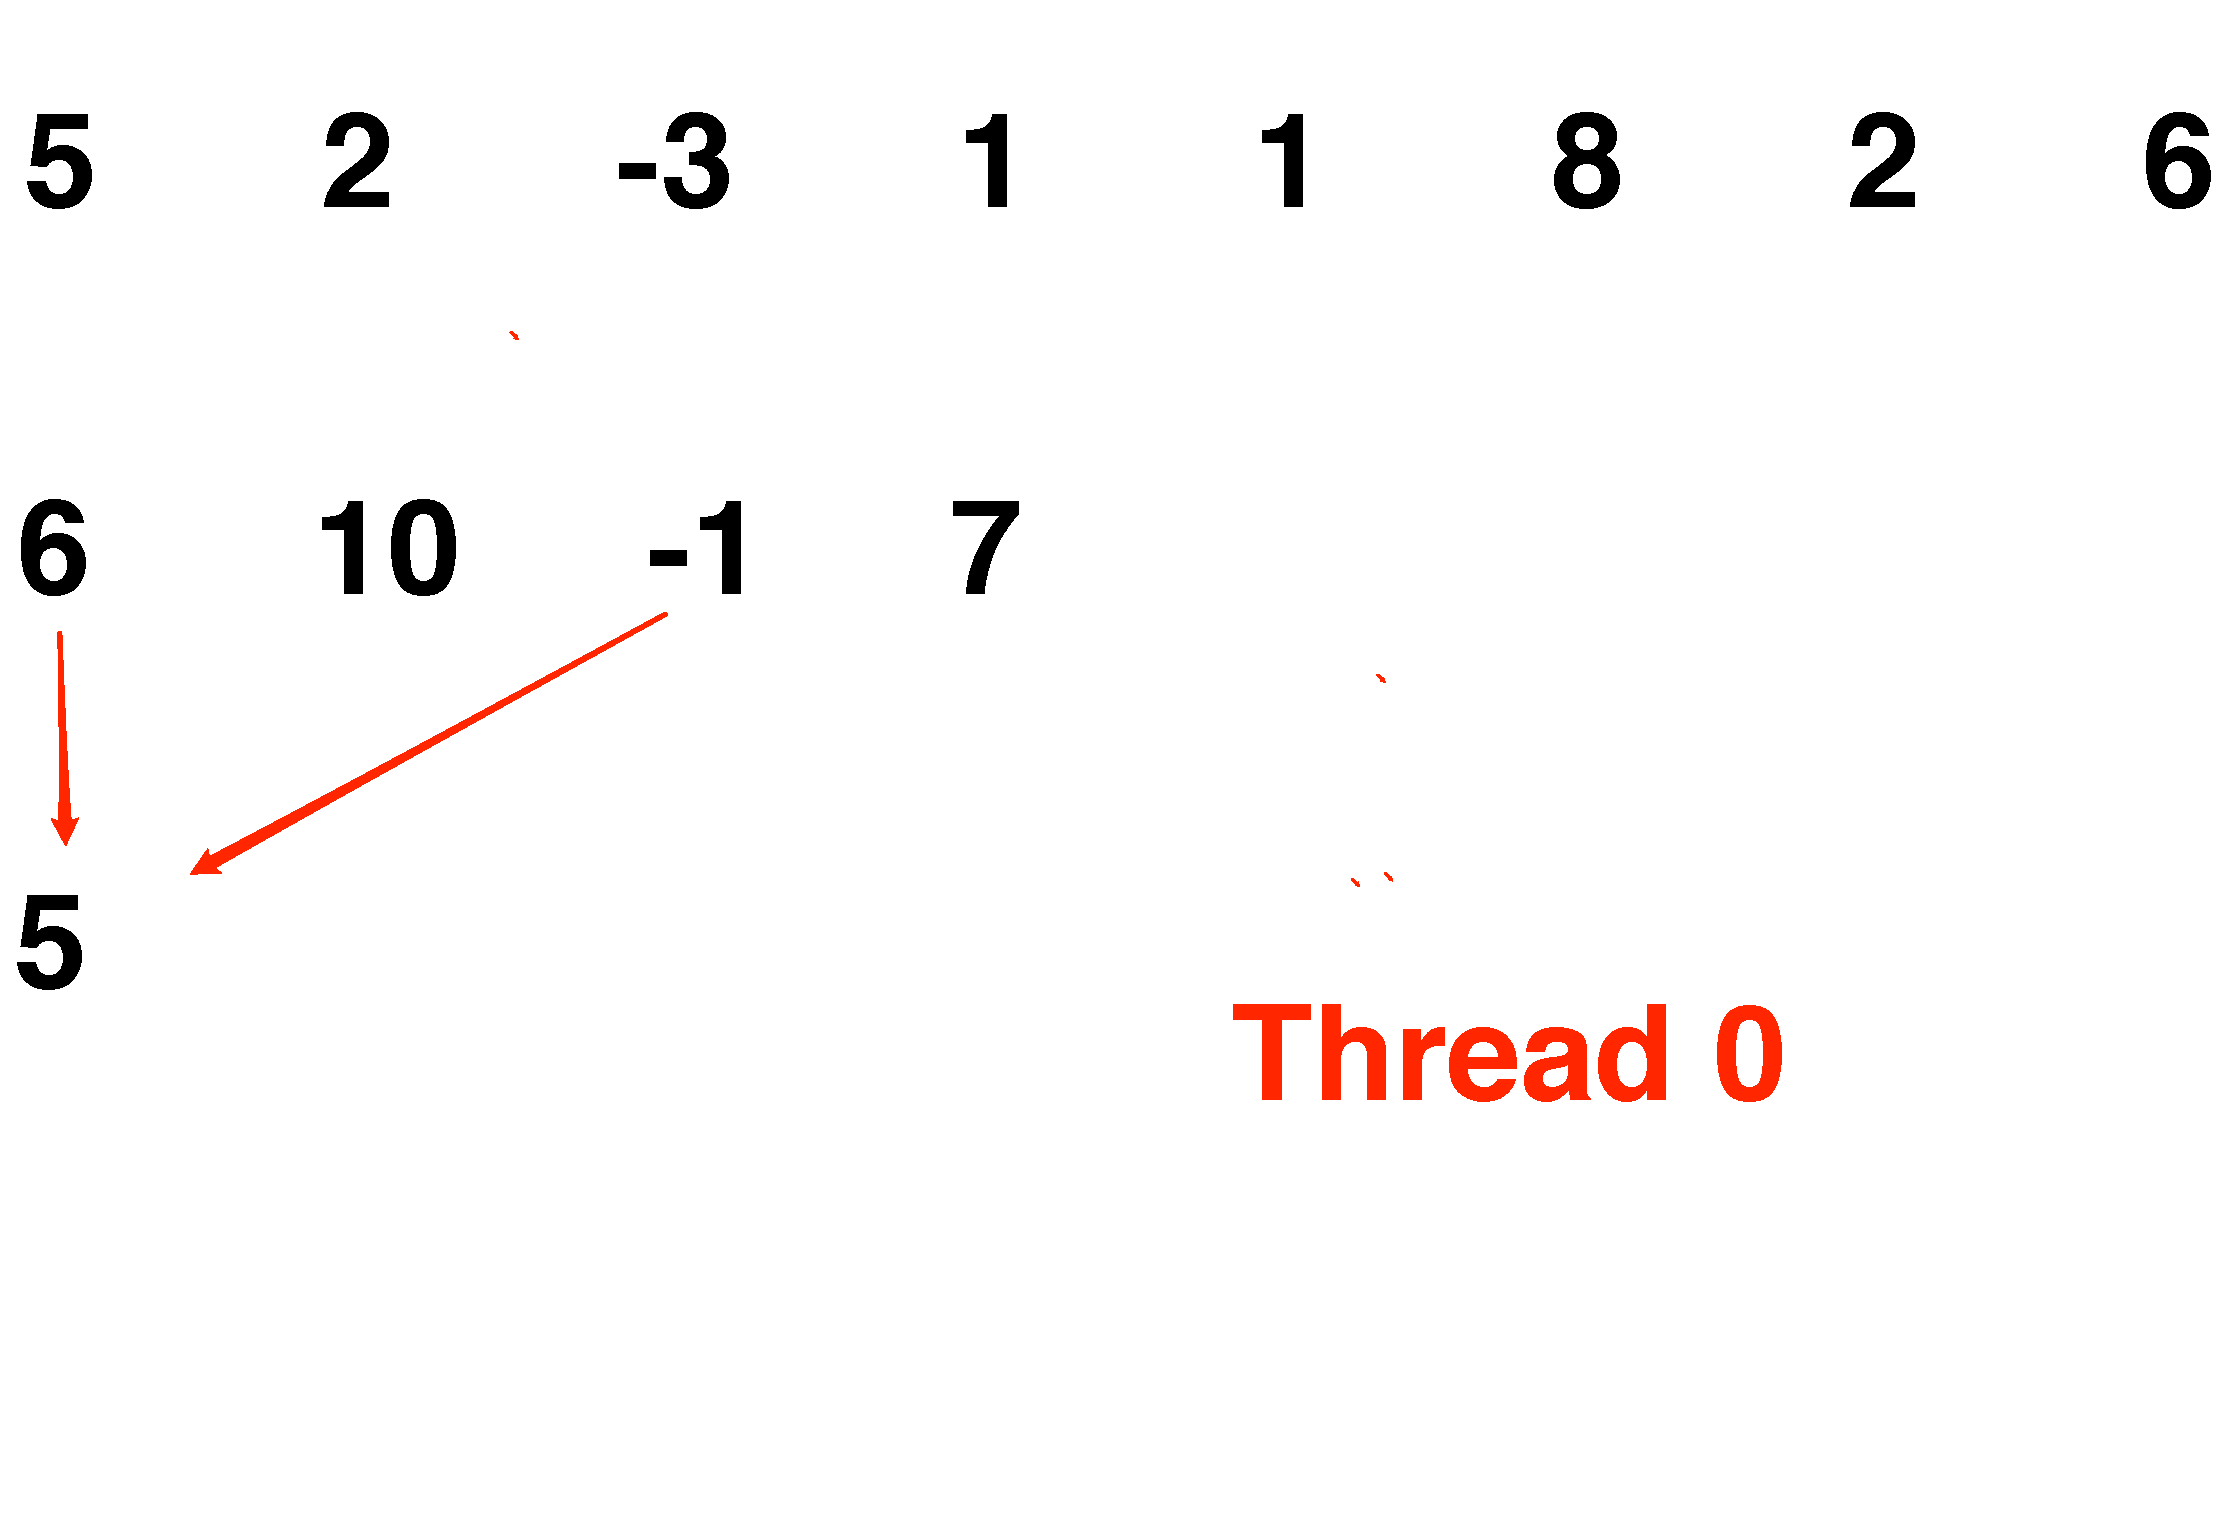
\includegraphics[scale=.25]{fig/psum6.pdf}
\end{frame}

\begin{frame}
\frametitle{Pairwise summation: an example reduction}
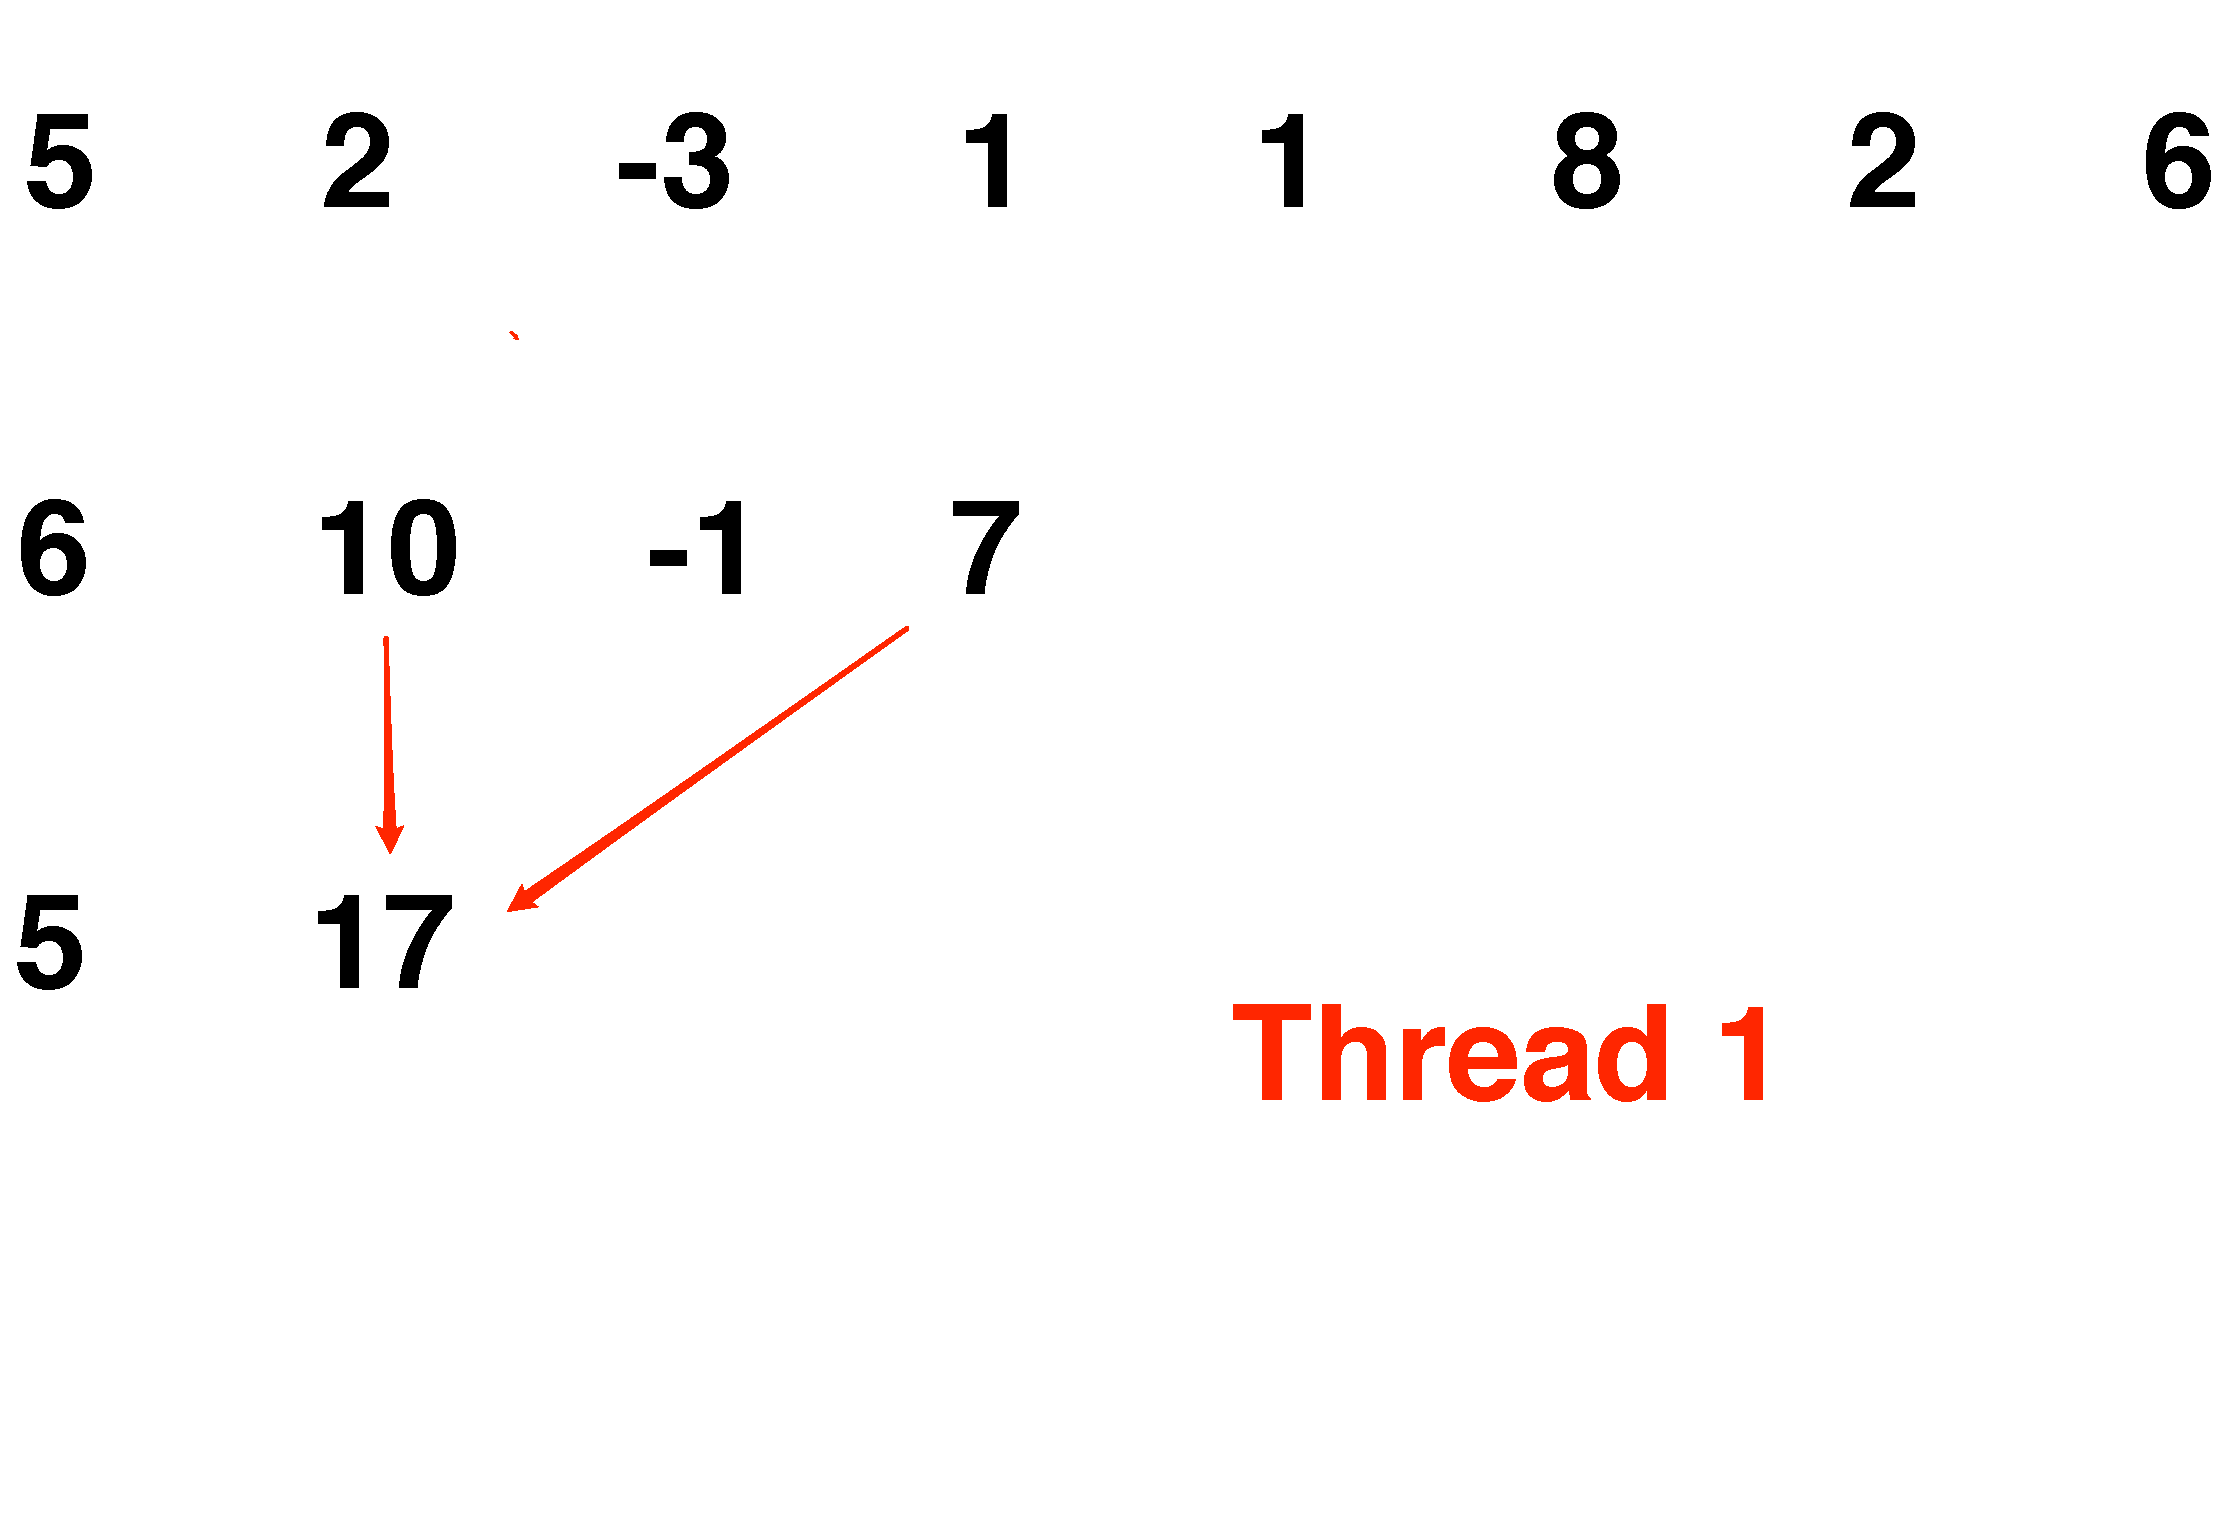
\includegraphics[scale=.25]{fig/psum7.pdf}
\end{frame}

\begin{frame}
\frametitle{Pairwise summation: an example reduction}
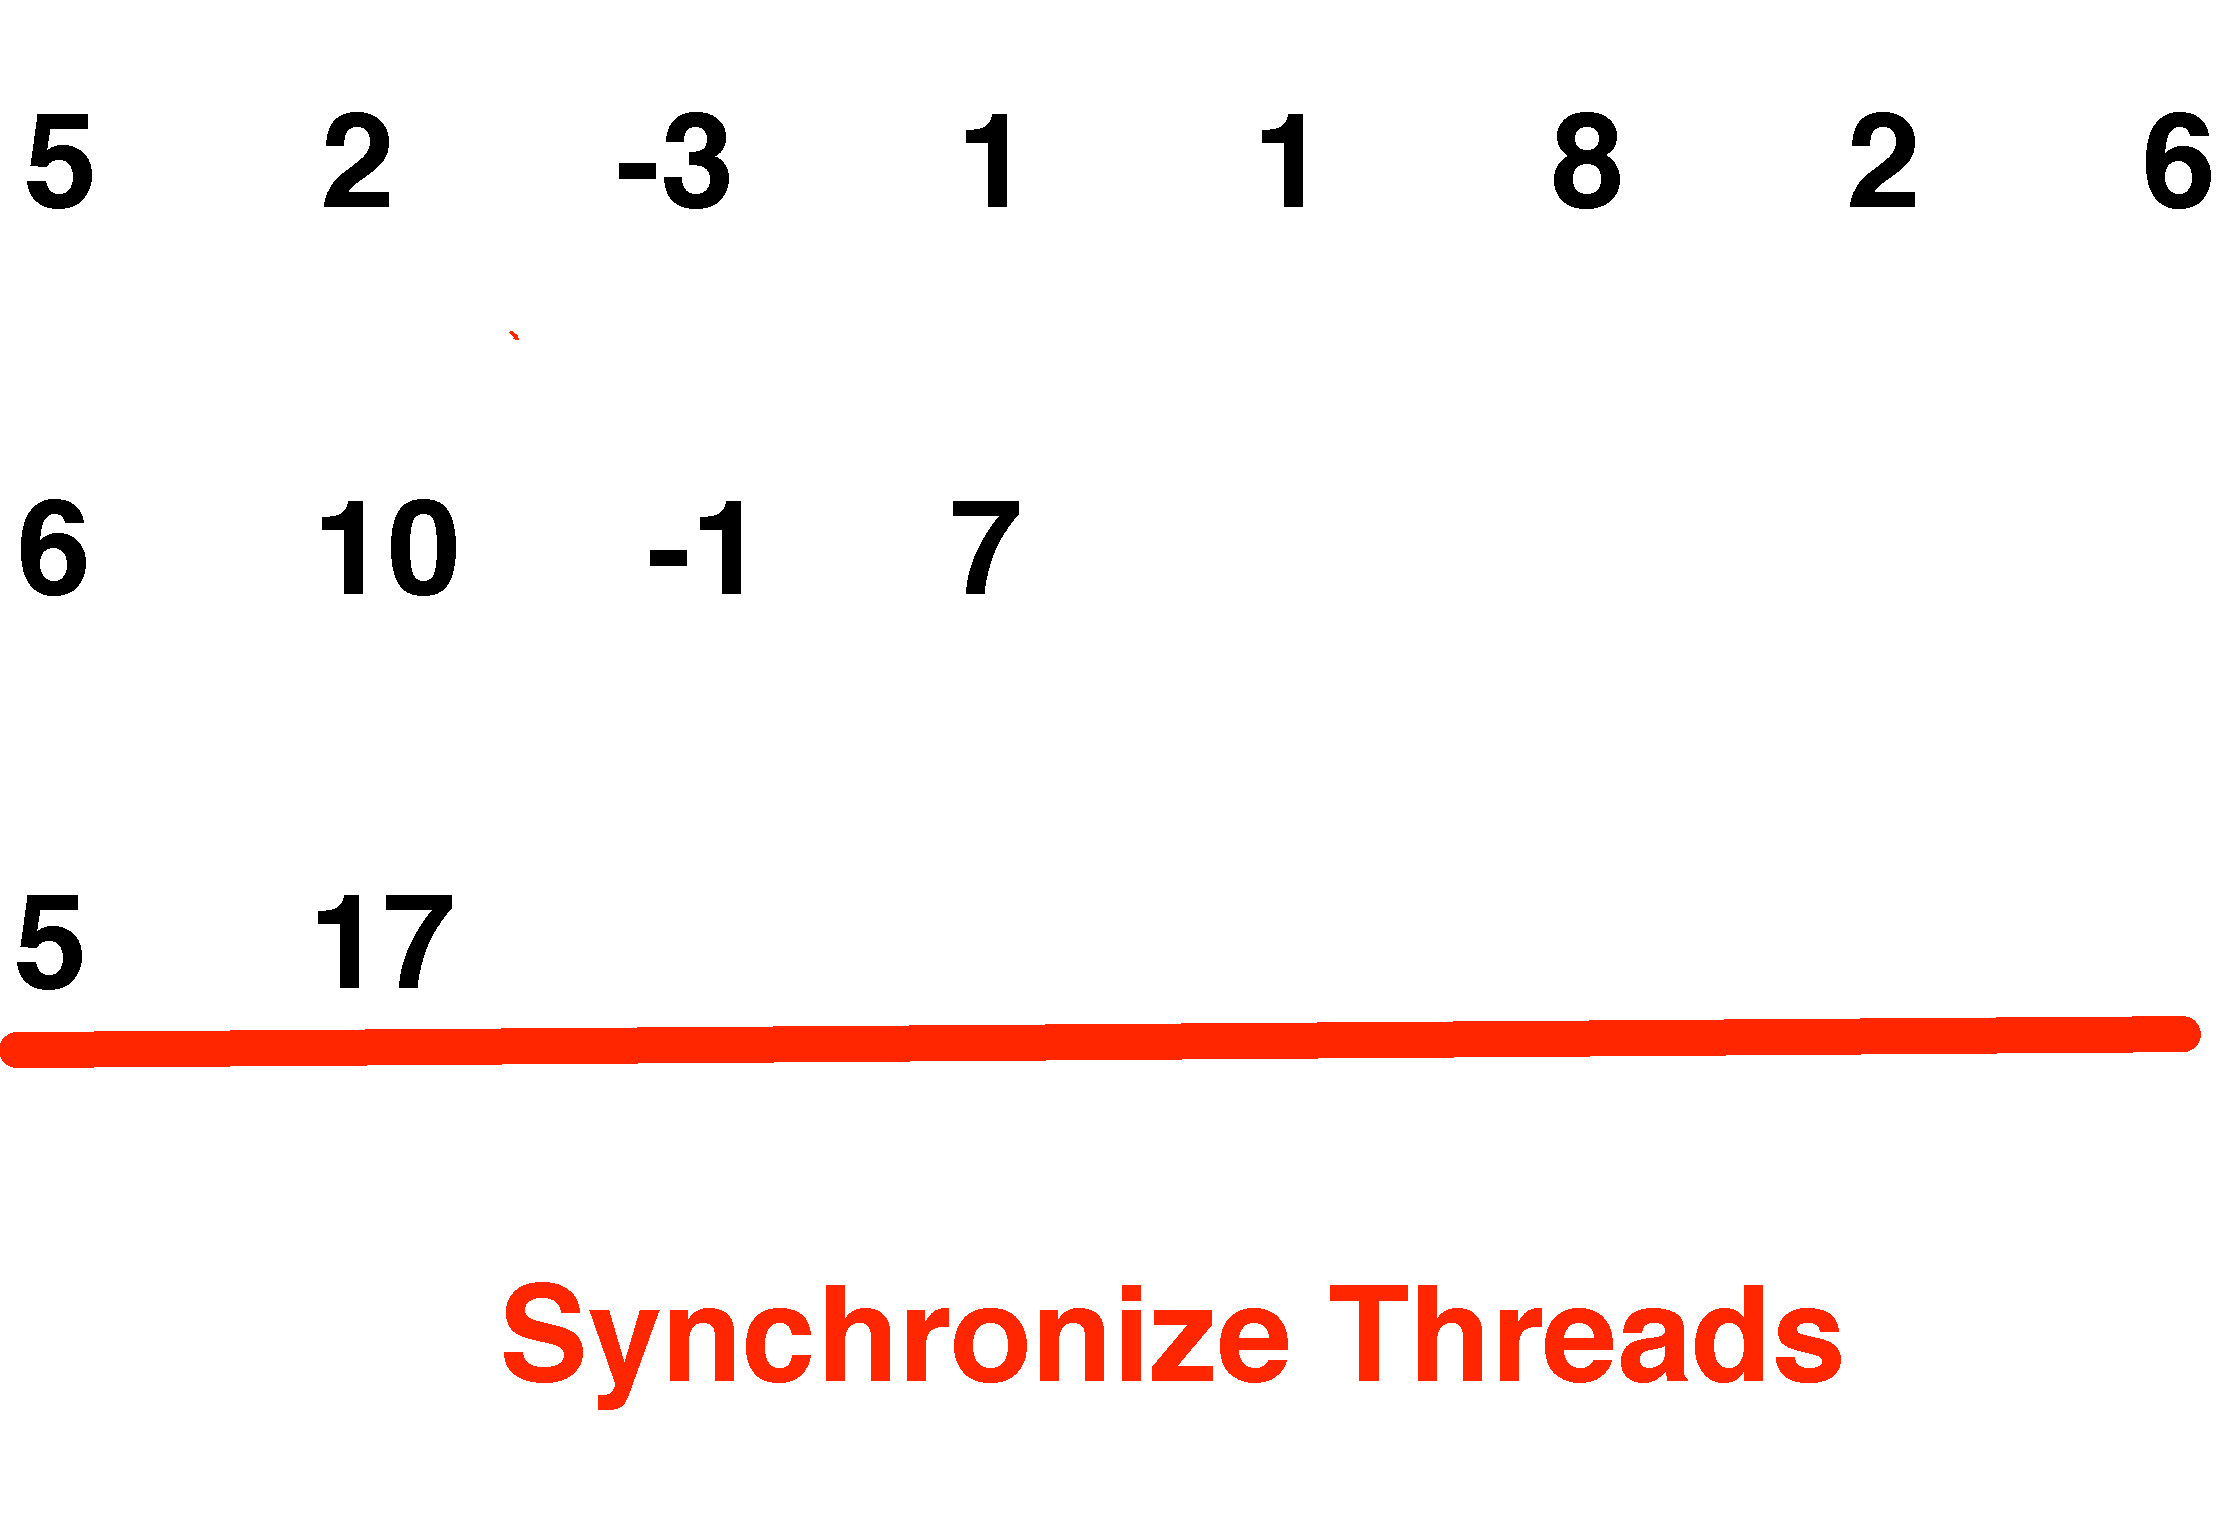
\includegraphics[scale=.25]{fig/psum8.pdf}
\end{frame}

\begin{frame}
\frametitle{Pairwise summation: an example reduction}
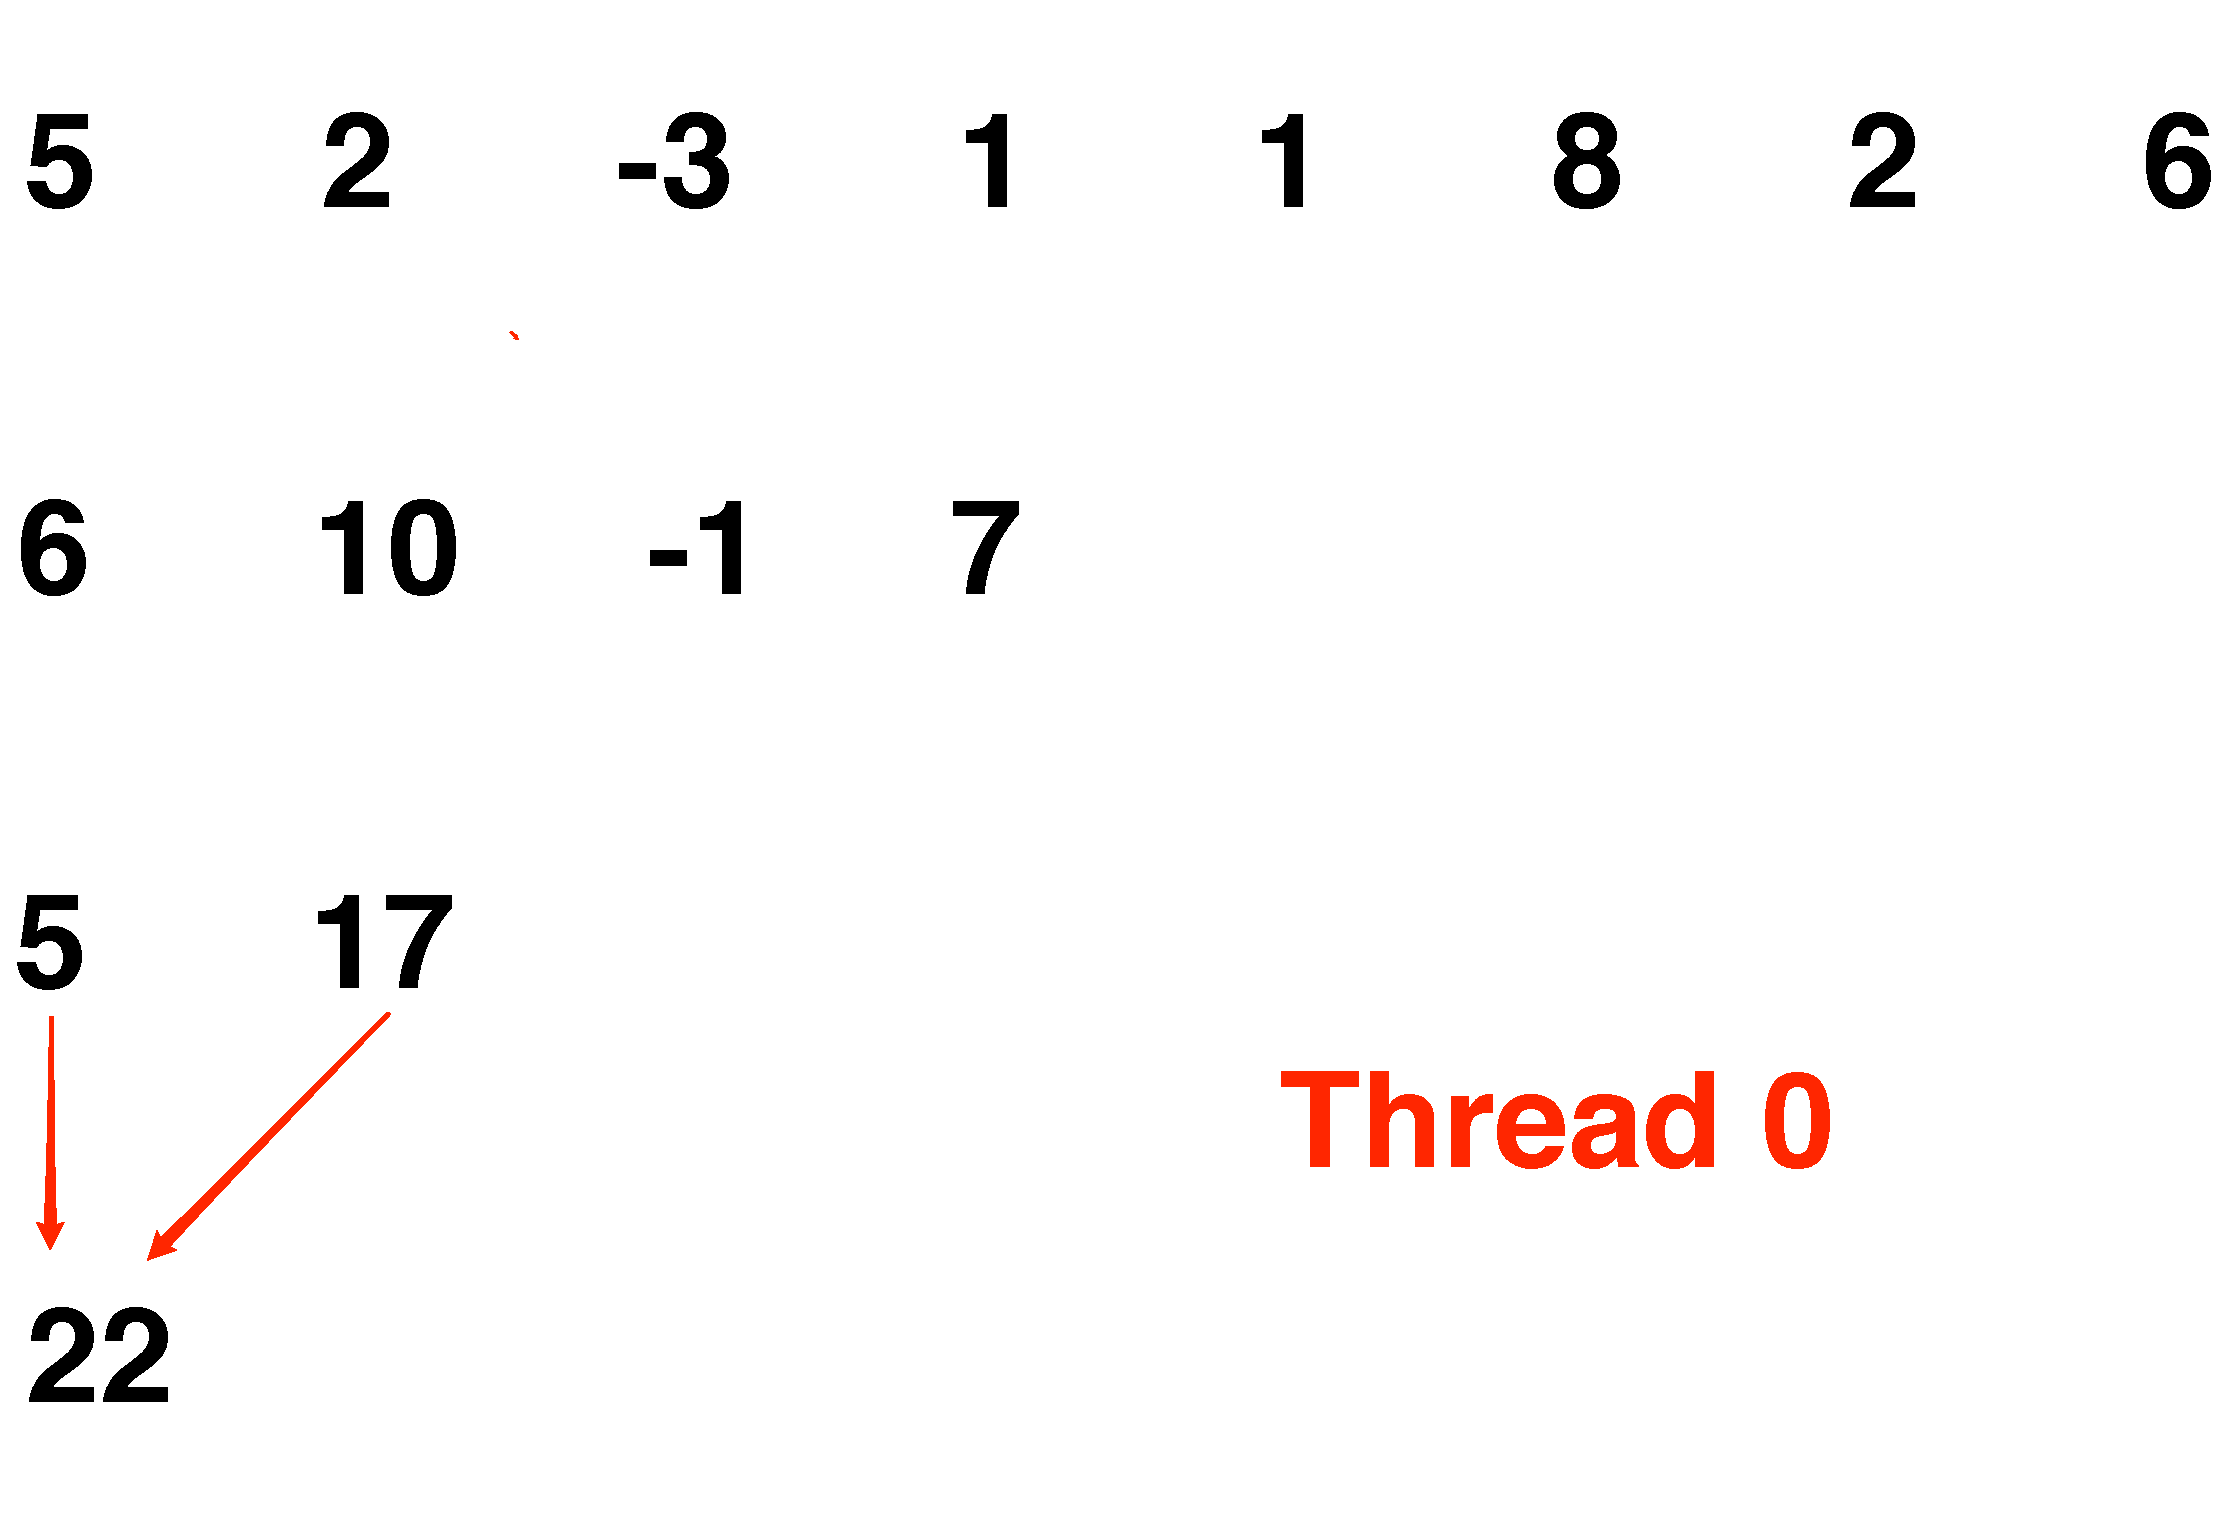
\includegraphics[scale=.25]{fig/psum9.pdf}
\end{frame}







\begin{frame}
\frametitle{Example: $\tau^2$} \scriptsize
\begin{align*}
&y_{g,n} \stackrel{\text{ind}}{\sim} \text{Poisson}( \exp(c_n + \e_{g, n} + \mu(n, \phi_g, \alpha_g, \delta_g))) \\
& \qquad \uncover<2->{ \e_{g, n} \stackrel{\text{ind}}{\sim} \text{N}( 0, \eta_g^2)} \\
& \qquad \qquad \uncover<3->{\eta_g^2 \stackrel{\text{ind}}{\sim} \text{Inv-Gamma}\left (\left . \text{shape} = \frac{d}{2} \right ., \ \text{rate} =  \frac{d \cdot \tau^2}{2} \right)} \\
& \qquad \qquad \qquad \uncover<4->{d \stackrel{\text{}}{\sim} \text{U}( 0, d_0)} \\
& \qquad \qquad \qquad \uncover<5->{\tau^2 \stackrel{\text{}}{\sim} \text{Gamma}( \text{shape} = a_\tau, \text{rate} = b_\tau)} \\
\uncover<6->{p(\tau^2 & \mid \cdots)}  \\
&\uncover<6->{= \text{Gamma} \left ( \left . \text{shape} =  a_\tau + \frac{Gd}{2} \right ., \ \text{rate} =  b_\tau + \frac{d}{2} {\color{blue} \sum_{g = 1}^G \frac{1}{\eta_g^2}} \right ) }
\end{align*}

\begin{itemize}
\uncover<7->{\item Using a parallel reduction (NVIDIA's CUDA C/C++ {\tt Thrust} library), calculate the sufficient statistic:}
\begin{align*}
\uncover<8->{\color{blue}\sum_{g = 1}^G \frac{1}{\eta_g^2}}
\end{align*}
\uncover<9->{\item Use an efficient rejection sampler to sample $\tau^2$.}
\end{itemize}

\end{frame}




\begin{frame}
\frametitle{Example: $d$} \tiny
\begin{align*}
&y_{g,n} \stackrel{\text{ind}}{\sim} \text{Poisson}( \exp(c_n + \e_{g, n} + \mu(n, \phi_g, \alpha_g, \delta_g))) \\
& \qquad \uncover<2->{ \e_{g, n} \stackrel{\text{ind}}{\sim} \text{N}( 0, \eta_g^2)} \\
& \qquad \qquad \uncover<3->{\eta_g^2 \stackrel{\text{ind}}{\sim} \text{Inv-Gamma}\left (\left . \text{shape} = \frac{d}{2} \right ., \ \text{rate} =  \frac{d \cdot \tau^2}{2} \right)} \\
& \qquad \qquad \qquad \uncover<4->{d \stackrel{\text{}}{\sim} \text{U}( 0, d_0)} \\
& \qquad \qquad \qquad \uncover<5->{\tau^2 \stackrel{\text{}}{\sim} \text{Gamma}(\text{shape} = a_\tau, \text{rate} = b_\tau)} \\
&\uncover<6->{p(d \mid \cdots) \propto \Gamma \left( d/2 \right )^{-G} \left ( \frac{d \cdot \tau^2}{2}\right ) ^ { G d  /2 } \left ({\color{blue} \prod_{g = 1}^G { \eta_g^2} } \right )^{ -(d/2 + 1)} \exp \left (- \frac{d \cdot \tau^2}{2} {\color{blue} \sum_{g = 1}^G \frac{1}{ \eta_g^2} }\right ) I(0 < d < d_0) }
\end{align*}



\small
\begin{itemize}
\uncover<7->{\item Using parallel reductions (NVIDIA's CUDA C/C++ {\tt Thrust} library), calculate the sufficient statistics:}
\begin{align*}
\uncover<8->{\color{blue}\prod_{g = 1}^G \eta_g^2 \qquad \qquad \sum_{g = 1}^G \frac{1}{\eta_g^2} } 
\end{align*}
\uncover<9->{\item Use a random-walk metropolis step to sample $d$.}
\end{itemize}
\end{frame}






\section{The software}

\setcounter{subsection}{1}


\begin{frame}
\frametitle{The software}
\begin{itemize}
\item In progress...
\end{itemize}

\end{frame}


\begin{frame}
\frametitle{Thanks for coming.}
\begin{itemize}
\item Slides and video will be available at \url{http://will-landau.com/research.html}.
\end{itemize}
\end{frame}

\begin{frame}
\frametitle{Sources}
\begin{enumerate}[1. ]
\item A. Gelman, J. B. Carlin, H. S. Stern, and D. S. Rubin. Bayesian Data Analysis. Chapman \& Hall/CRC, 2 edition, 2004.
\item Prof. Jarad Niemi's STAT 544 lecture notes.
\item J. Sanders and E. Kandrot. \emph{CUDA by Example.} Addison-Wesley, 2010.
\item \url{http://www.astrochem.org/sci/Nucleobases.php}
\item \url{http://www.biologycorner.com/bio1/DNA.html}
\item \url{http://www.qualitysilks.com/images/products/artificial-corn-stalk.jpg}
\item \url{http://en.wikipedia.org/wiki/dna}
\item \url{http://en.wikipedia.org/wiki/rna}
\item \url{http://en.wikipedia.org/wiki/HSP60}
\end{enumerate}
\end{frame}

\end{document}